\documentclass[master, english]{ihethesis}

\usepackage[nottoc,chapter]{tocbibind}					% Add bibliography/index/contents to Table of Contents
\usepackage{microtype}									% Subliminal refinements towards typographical perfection
\usepackage{booktabs}									% The pack­age en­hances the qual­ity of ta­bles in LaTeX
\usepackage{tabularx}									% Tabulars with adjustable-width columns
\usepackage{floatrow}									% Modifying the layout of floats
\floatsetup[table]{capposition=top}
\floatsetup[figure]{font=footnotesize}
\usepackage{romannum}									% Generate roman numerals instead of arabic digits				
\usepackage{amsmath}									% AMS mathematical facilities for LaTeX
\usepackage{amssymb}									% TeX fonts from the American Mathematical Society

\usepackage{import}

\usepackage[product-units = single, multi-part-units = brackets, detect-all, load-configurations=abbreviations, range-units = repeat, separate-uncertainty = false, per-mode=symbol]{siunitx} 			% Correct use of SI units
%\newcommand{\SIp}[2]{\SI[product-units = power]{#1}{#2}} % p for power (chip size...)
%\newcommand{\SIrangem}[2]{\SIrange[range-phrase = --]{#1}{#2}}
%\newcommand{\SIrangecp}[2]{\SIrange[range-phrase = --, range-units = brackets, output-complex-root = j, complex-root-position = before-number]{#1}{#2}}
%\sisetup{separate-uncertainty}%
\newcommand{\SIr}{\SIrange[range-units = single]}

\usepackage{epstopdf}									% Convert EPS to 'encapsulated' PDF using Ghostscript
\usepackage[small]{caption}								% Customising captions in floating environments
%\usepackage{subcaption}
%\usepackage{transparent}
\usepackage[percent]{overpic}							% Combine LaTeX commands over included graphics
\usepackage[title,header]{appendix}						% Extra control of appendices
%\renewcommand{\appendixpagename}{Anhang}
%\usepackage[usenames,dvipsnames,svgnames,table]{xcolor}
\usepackage{color}										% Colour control for LaTeX documents
\usepackage{subfig}
% Hoehe des Headings anpassen um Fehlermeldung zu unterdrücken, ansonsten folgende zeile wieder löschen:
\setlength{\headheight}{1.5\baselineskip}

\mathchardef\mhyphen="2D
\definecolor{grey}{RGB}{228,228,228}

%\usepackage[pdftex
%            %,colorlinks
%            ,hidelinks %% keine roten Rahmen um Links
%            ,hyperindex
%            ,plainpages=false
%            ,bookmarksopen
%            ,bookmarksnumbered]{hyperref}
%            
%\hypersetup{
%pdftitle={\@title},
%pdfauthor={\@author},
%pdfsubject={\@title},
%%,pdfborder={0 0 0}
%%colorlinks=true,
%%linkcolor=red,          % color of internal links
%%citecolor=black,        % color of links to bibliography
%%filecolor=black,      % color of file links
%%urlcolor=black           % color of external links
%}															

\usepackage[acronym, 
						nonumberlist, 
						toc, 
						nopostdot, 
						style=alttree, 
						nogroupskip]
												{glossaries}
% Nopostdot omits dots at the end of each entry, alttree makes two columns (use \glssetwidest), alternative style=long, nogroupskip no groups by first letter

\setacronymstyle{short-long}
\glssetwidest{$L_{\left(C-package\right)_{eff}}$}% widest name
\renewcommand*{\glsnamefont}[1]{\textmd{#1}} % Define font of entry name
%%%
%%% Abbreviations %%%double-sideband
%%%
\newglossary[abg]{abbreviations}{ab}{abn}{List of abbreviations}
%

\newglossaryentry{ab:sqnr}{type=abbreviations,name={SQNR},description={Signal-to-quantization-noise-ratio},first={SQNR (Signal-to-quantization-noise-ratio)}}


\newglossaryentry{ab:2deg}{type=abbreviations,name={2DEG},description={Two-dimensional electron gas},first={2DEG (two-dimensional electron gas)},firstplural={2DEGs (two-dimensional electron gases)},plural={2DEGs}}

\newglossaryentry{ab:ads}{type=abbreviations,name={ADS},description={Advanced Design System},first={ADS (Advanced Design System)}}

\newglossaryentry{ab:dac}{type=abbreviations,name={DAC},description={digital-to-analog converter},first={DAC (digital-to-analog converter)}}

\newglossaryentry{ab:osr}{type=abbreviations,name={OSR},description={oversampling ratio},first={OSR (oversampling ratio)}}

\newglossaryentry{ab:iaf}{type=abbreviations,name={IAF},description={Fraunhofer-Institut f\"ur Angewandte Festk\"orperphysik}}

\newglossaryentry{ab:de}{type=abbreviations,name={DE},description={drain efficiency},first={DE (drain efficiency)},firstplural={DEs (drain efficiencies)},plural={DEs}}

\newglossaryentry{ab:de_max}{type=abbreviations,name={DE$_{max}$},description={maximum drain efficiency},first={DE$_{max}$ (maximum drain efficiency)},firstplural={DE$_max$s (maximum drain efficiencies)},plural={DE$_max$s}}
\newglossaryentry{ab:pae}{type=abbreviations,name={PAE},description={power-added efficiency},first={PAE (power-added efficiency)},firstplural={PAEs (power-added efficiencies)},plural={PAEs}}
\newglossaryentry{ab:pae_max}{type=abbreviations,name={PAE$_{max}$},description={maximum power-added efficiency},first={PAE$_{max}$ (maximum power-added efficiency)},firstplural={PAE$_max$s (maximum power-added efficiencies)},plural={PAE$_max$s}}
\newglossaryentry{ab:pa}{type=abbreviations,name={PA},description={power amplifier},first={PA (power amplifier)},firstplural={PAs (power amplifiers)},plural={PAs}}
\newglossaryentry{ab:hpa}{type=abbreviations,name={HPA},description={high power amplifier},first={HPA (high power amplifier)},firstplural={HPAs (high power amplifiers)},plural={HPAs}}
\newglossaryentry{ab:gan}{type=abbreviations,name={GaN},description={gallium nitride},first={GaN (gallium nitride)}}
\newglossaryentry{ab:algan}{type=abbreviations,name={AlGaN},description={aluminium gallium nitride},first={AlGaN (aluminium gallium nitride)}}
\newglossaryentry{ab:gaas}{type=abbreviations,name={GaAs},description={gallium arsenide},first={GaAs (gallium arsenide)}}
\newglossaryentry{ab:inp}{type=abbreviations,name={InP},description={indium phosphide},first={InP (indium phosphide)}}
\newglossaryentry{ab:sic}{type=abbreviations,name={SiC},description={silicon carbide},first={SiC (silicon carbide)}}
\newglossaryentry{ab:si}{type=abbreviations,name={Si},description={silicon},first={Si (silicon)}}
\newglossaryentry{ab:sapphire}{type=abbreviations,name={Al$_2$0$_3$},description={sapphire},first={Al$_2$0$_3$ (sapphire)}}
\newglossaryentry{ab:ldmos}{type=abbreviations,name={LDMOS},description={laterally diffused metal oxide semiconductor},first={LDMOS (laterally diffused metal oxide semiconductor)}}
\newglossaryentry{ab:hemt}{type=abbreviations,name={HEMT},description={high electron mobility transistor},first={HEMT (high electron mobility transistor)},firstplural={HEMTs (high electron mobility transistors)},plural={HEMTs}}
\newglossaryentry{ab:mmic}{type=abbreviations,name={MMIC},description={microwave monolithic integrated circuit},first={MMIC (microwave monolithic integrated circuit)},firstplural={MMICs (microwave monolithic integrated circuits)},plural={HEMTs}}
\newglossaryentry{ab:lte}{type=abbreviations,name={LTE},description={Long-Term Evolution},first={LTE (Long-Term Evolution)}}
\newglossaryentry{ab:cmos}{type=abbreviations,name={CMOS},description={complementary metal-oxide-semiconductor},first={CMOS (complementary metal-oxide-semiconductor)}}
\newglossaryentry{ab:mos}{type=abbreviations,name={MOS},description={metal-oxide-semiconductor},first={MOS (metal-oxide-semiconductor)}}
\newglossaryentry{ab:bwi}{type=abbreviations,name={BWI},description={bondwire interconnect},first={BWI (bondwire interconnect)},firstplural={BWIs (bondwire interconnects)},plural={BWIs}}
\newglossaryentry{ab:msg}{type=abbreviations,name={MSG},description={maximum stable gain},first={MSG (maximum stable gain)}}
\newglossaryentry{ab:mag}{type=abbreviations,name={MAG},description={maximum available gain},first={MAG (maximum available gain)}}
\newglossaryentry{ab:imn}{type=abbreviations,name={IMN},description={input matching network},first={IMN (input matching network)}}
\newglossaryentry{ab:omn}{type=abbreviations,name={OMN},description={output matching network},first={OMN (output matching network)}}
\newglossaryentry{ab:dc}{type=abbreviations,name={DC},description={direct current},first={DC (direct current)}}
\newglossaryentry{ab:rf}{type=abbreviations,name={RF},description={radio frequency},first={RF (radio frequency)}}
\newglossaryentry{ab:msl}{type=abbreviations,name={MSL},description={microstrip line},first={MSL (microstrip line)},firstplural={MSLs (microstrip lines)},plural={MSLs}}
\newglossaryentry{ab:tl}{type=abbreviations,name={TL},description={transmission line},first={TL (transmission line)},firstplural={TLs (transmission lines)},plural={TLs}}
\newglossaryentry{ab:cs}{type=abbreviations,name={CS},description={common-source},first={CS (common-source)}}
\newglossaryentry{ab:ippm}{type=abbreviations,name={IPPM},description={in-package pre-matching},first={IPPM (in-package pre-matching)}}
\newglossaryentry{ab:plc}{type=abbreviations,name={PLC},description={package-lead-compensation},first={PLC (package-lead-compensation)}}
\newglossaryentry{ab:esr}{type=abbreviations,name={ESR},description={equivalent series resistance},first={ESR (equivalent series resistance)}}
\newglossaryentry{ab:nicr}{type=abbreviations,name={NiCr},description={nickel chromium},first={NiCr (nickel chromium)}}
\newglossaryentry{ab:sp}{type=abbreviations,name={S-parameters},description={scattering parameters},first={S-parameters (scattering parameters)}}
\newglossaryentry{ab:il}{type=abbreviations,name={IL},description={logarithmic insertion loss},first={IL (logarithmic insertion loss)}}
\newglossaryentry{ab:em}{type=abbreviations,name={EM},description={electromagnetic},first={EM (electromagnetic)}}
\newglossaryentry{ab:SP}{type=abbreviations,name={SP},description={S-Parameter simulation controller},first={SP (S-Parameter simulation controller)}}
\newglossaryentry{ab:HB}{type=abbreviations,name={HB},description={Harmonic Balance simulation controller},first={HB (Harmonic Balance simulation controller)}}
\newglossaryentry{ab:dut}{type=abbreviations,name={DUT},description={device under test},first={DUT (device under test)}}
\newglossaryentry{ab:cw}{type=abbreviations,name={CW},description={continuous wave},first={CW (continuous wave)}}
\newglossaryentry{ab:wcdma}{type=abbreviations,name={WCDMA},description={Wideband Code Division Multiple Access},first={WCDMA (Wideband Code Division Multiple Access)}}
\newglossaryentry{ab:im3}{type=abbreviations,name={IM3},description={third order intercept point},first={IM3 (third order intercept point)}}
\newglossaryentry{ab:acpr}{type=abbreviations,name={ACPR},description={adjacent channel power ratio},first={ACPR (adjacent channel power ratio)}}
\newglossaryentry{ab:pbo}{type=abbreviations,name={PBO},description={power back-off},first={PBO (power back-off)}}







%%%
%%% Symbols %%%
%%%
\newglossary[slg]{symbols}{sy}{sbl}{List of symbols}
%
\newglossaryentry{sy:freq}{type=symbols,name={$f$},description={frequency},first={$f$ (frequency)}}
\newglossaryentry{sy:V}{type=symbols,name={$V$},description={Voltage},first={$V$ (Voltage)}}
\newglossaryentry{sy:VDS}{type=symbols,name={$V_{DS}$},description={DC-component of the drain source voltage},first={$V_{DS}$ (DC-component of the drain source voltage)}}
\newglossaryentry{sy:VGS}{type=symbols,name={$V_{GS}$},description={DC-component of the gate source voltage},first={$V_{GS}$ (DC-component of the gate source voltage)}}
\newglossaryentry{sy:vds}{type=symbols,name={$v_{ds}$},description={RF-component of the drain source voltage},first={$v_{ds}$ (RF-component of the drain source voltage)}}
\newglossaryentry{sy:vds_peak}{type=symbols,name={$\hat{v_{ds}}$},description={peak value of the RF-component of the drain source voltage},first={$\hat{v_{ds}}$} (peak value of the RF-component of the drain source voltage)}
\newglossaryentry{sy:ID}{type=symbols,name={$I_D$},description={DC-component of the drain current},first={$I_D$ (DC-component of the drain current)}}
\newglossaryentry{sy:pout}{type=symbols,name={$P_{out}$},description={RF output power},first={$P_{out}$ (RF output power)}}
\newglossaryentry{sy:pout_max}{type=symbols,name={$P_{out_{max}}$},description={maximum RF output power},first={$P_{out_{max}}$ (maximum RF output power)}}
\newglossaryentry{sy:pout_lin}{type=symbols,name={$P_{out_{lin}}$},description={maximum linear RF output power},first={$P_{out_{lin}}$ (maximum linear RF output power)}}
\newglossaryentry{sy:pout_avail}{type=symbols,name={$P_{out_{avail}}$},description={RF output power available from the generator},first={$P_{out_{avail}}$ (RF output power available from the generator)}}
\newglossaryentry{sy:pout_del}{type=symbols,name={$P_{out_{del}}$},description={RF output power delivered to load},first={$P_{out_{del}}$ (RF output power delivered to load)}}
\newglossaryentry{sy:pdc}{type=symbols,name={$P_{DC}$},description={consumed DC power},first={$P_{DC}$ (consumed DC power)}}
\newglossaryentry{sy:pin}{type=symbols,name={$P_{in}$},description={RF input power},first={$P_{in}$ (RF input power)}}
\newglossaryentry{sy:pin4db}{type=symbols,name={$P_{in_{4dB}}$},description={RF input power yielding 4 dB of gain compression},first={$P_{in_{4dB}}$ (RF input power yielding 4 dB of gain compression)}}
\newglossaryentry{sy:cgs}{type=symbols,name={$C_{gs}$},description={gate source capacitance},first={$C_{gs}$ (gate source capacitance)}}
\newglossaryentry{sy:cgd}{type=symbols,name={$C_{gd}$},description={gate drain capacitance},first={$C_{gd}$ (gate drain capacitance)}}
\newglossaryentry{sy:cds}{type=symbols,name={$C_{ds}$},description={drain source capacitance},first={$C_{ds}$ (drain source capacitance)}}
\newglossaryentry{sy:ccomp}{type=symbols,name={$C_{comp}$},description={in-package shunt compensation capacitance},first={$C_{comp}$ (in-package shunt compensation capacitance)}}
\newglossaryentry{sy:qn}{type=symbols,name={$Q_n$},description={nodal quality factor},first={$Q_n$ (nodal quality factor)}}
\newglossaryentry{sy:qn_max}{type=symbols,name={$Q_{n_{max}}$},description={maximum nodal quality factor of a network},first={$Q_{n_{max}}$ (maximum nodal quality factor of a network)}}
\newglossaryentry{sy:ql}{type=symbols,name={$Q_L$},description={loaded quality factor},first={$Q_L$ (loaded quality factor)}}
\newglossaryentry{sy:zin}{type=symbols,name={$Z_{in}$},description={input impedance},first={$Z_{in}$ (input impedance)}}
\newglossaryentry{sy:rin}{type=symbols,name={$R_{in}$},description={input resistance},first={$R_{in}$ (input resistance)}}
\newglossaryentry{sy:zout}{type=symbols,name={$Z_{out}$},description={output impedance},first={$Z_{out}$ (output impedance)}}
\newglossaryentry{sy:zin_pb}{type=symbols,name={$Z_{in_{PB}}$},description={input impedance of the powerbar},first={$Z_{in_{PB}}$ (input impedance of the powerbar)}}
\newglossaryentry{sy:z_pb+lead}{type=symbols,name={$Z_{PB+lead}$},description={impedance seen from the package-lead towards the packaged powerbar},first={$Z_{PB+lead}$ (impedance seen from the package-lead towards the packaged powerbar)}}
\newglossaryentry{sy:z_ref_plane}{type=symbols,name={$Z_{ref plane}$},description={impedance seen from the package reference plane towards the packaged powerbar},first={$Z_{ref plane}$ (impedance seen from the package reference plane towards the packaged powerbar)}}
\newglossaryentry{sy:zn}{type=symbols,name={$Z_n$},description={nodal impedance seen from a node into a network},first={$Z_n$ (nodal impedance seen from a node into a network)}}
\newglossaryentry{sy:X_n}{type=symbols,name={$\left|X_n\right|$},description={absolute value of the imaginary part of the impedance seen at the node},first={$\left|X_n\right|$ (absolute value of the imaginary part of the impedance seen at the node)}}
\newglossaryentry{sy:R_n}{type=symbols,name={$R_n$},description={real part of the impedance seen at the node},first={$R_n$ (real part of the impedance seen at the node)}}
\newglossaryentry{sy:bw}{type=symbols,name={$BW$},description={absolute bandwidth},first={$BW$ (absolute bandwidth)}}
\newglossaryentry{sy:f0}{type=symbols,name={$f_0$},description={centre frequency},first={$f_0$ (centre frequency)}}
\newglossaryentry{sy:l_pb_c}{type=symbols,name={$L_{\left(PB-C\right)_{eff}}$},description={effective inductance from the powerbar gate to the \gls{ab:mos}-capacitor},first={$L_{\left(PB-C\right)_{eff}}$ (effective inductance from the powerbar gate to the \gls{ab:mos}-capacitor)}}
\newglossaryentry{sy:l_c_package}{type=symbols,name={$L_{\left(C-package\right)_{eff}}$},description={effective inductance from the \gls{ab:mos}-capacitor to the package},first={$L_{\left(C-package\right)_{eff}}$ (effective inductance from the \gls{ab:mos}-capacitor to the package)}}
\newglossaryentry{sy:trans_ratio}{type=symbols,name={$n_{trans}$},description={transformation ratio},first={$n_{trans}$ (transformation ratio)}}
\newglossaryentry{sy:id}{type=symbols,name={$i_d$},description={RF component of the drain current},first={$i_d$ (RF component of the drain current)}}
\newglossaryentry{sy:id_peak}{type=symbols,name={$\hat{i_d}$},description={peak value of the RF component of the drain current},first={$\hat{i_d}$ (peak value of the RF component of the drain current)}}
\newglossaryentry{sy:ig}{type=symbols,name={$i_g$},description={RF component of the gate current},first={$i_g$ (RF component of the gate current)}}
\newglossaryentry{sy:phase_id}{type=symbols,name={$\phi_{i_d}$},description={phase of the RF component of the drain current},first={$\phi_{i_d}$ (phase of the RF component of the drain current)}}
\newglossaryentry{sy:r_odd_g}{type=symbols,name={$R_{odd_g}$},description={odd-mode suppression resistor connecting the gates of neighbouring basecells},first={$R_{odd_g}$ (odd-mode suppression resistor connecting the gates of neighbouring basecells)}}
\newglossaryentry{sy:r_odd_d}{type=symbols,name={$R_{odd_d}$},description={odd-mode suppression resistor connecting the drains of neighbouring basecells},first={$R_{odd_d}$ (odd-mode suppression resistor connecting the drains of neighbouring basecells)}}
\newglossaryentry{sy:i_comp_g}{type=symbols,name={$i_{comp_g}$},description={compensation current flowing through $R_{odd_g}$ between the gates of neighbouring basecells},first={$i_{comp_g}$ (compensation current flowing through $R_{odd_g}$ between the gates of neighbouring basecells)}}
\newglossaryentry{sy:i_comp_d}{type=symbols,name={$i_{comp_d}$},description={compensation current flowing through $R_{odd_d}$ between the drains of neighbouring basecells},first={$i_{comp_d}$ (compensation current flowing through $R_{odd_d}$ between the drains of neighbouring basecells)}}
\newglossaryentry{sy:g_s}{type=symbols,name={$G(s)$},description={complex open loop transfer function},first={$G(s)$ (complex open loop transfer function)}}
\newglossaryentry{sy:gp}{type=symbols,name={$G_P$},description={power gain},first={$G_P$ (power gain)}}
\newglossaryentry{sy:gt}{type=symbols,name={$G_T$},description={transducer gain},first={$G_T$ (transducer gain)}}
\newglossaryentry{sy:fmax}{type=symbols,name={$f_{max}$},description={maximum frequency of oscillation},first={$f_{max}$ (maximum frequency of oscillation)}}
\newglossaryentry{sy:xc}{type=symbols,name={$X_C$},description={reactance of a capacitance},first={$X_C$ (reactance of a capacitance)}}
\newglossaryentry{sy:xl}{type=symbols,name={$X_L$},description={reactance of an inductance},first={$X_L$ (reactance of an inductance)}}
\newglossaryentry{sy:vth}{type=symbols,name={$V_{th}$},description={threshold voltage},first={$V_{th}$ (threshold voltage)}}
\newglossaryentry{sy:vgs}{type=symbols,name={$V_{gs}$},description={gate source voltage},first={$V_{gs}$ (gate source voltage)}}
\newglossaryentry{sy:rg}{type=symbols,name={$R_g$},description={effective gate resistance},first={$R_g$ (effective gate resistance)}}
\newglossaryentry{sy:delta_d}{type=symbols,name={$\Delta d$},description={displacement of the channel charge centroid away from the AlGaN/GaN contact interface},first={$\Delta d$ (displacement of the channel charge centroid away from the AlGaN/GaN contact interface)}}
\newglossaryentry{sy:zl}{type=symbols,name={$Z_{load}$},description={load impedance },first={$Z_{load}$ (load impedance)}}
\newglossaryentry{sy:zl_fs}{type=symbols,name={$Z_{load_{FS}}$},description={load impedance seen at full-scale drive},first={$Z_{load_{FS}}$ (load impedance at full-scale drive)}}
\newglossaryentry{sy:zl_6db}{type=symbols,name={$Z_{load_{-6dB}}$},description={load impedance seen at \SI{-6}{dB} PBO},first={$Z_{load_{-6dB}}$ (load impedance at \SI{-6}{dB} PBO)}}
\newglossaryentry{sy:rload}{type=symbols,name={$R_{load}$},description={load resistance },first={$R_{load}$ (load resistance)}}
\newglossaryentry{sy:xload}{type=symbols,name={$X_{load}$},description={load reactance},first={$X_{load}$ (load reactance)}}
\newglossaryentry{sy:gload}{type=symbols,name={$G_{load}$},description={load conductance},first={$G_{load}$ (load conductance)}}
\newglossaryentry{sy:bload}{type=symbols,name={$B_{load}$},description={load susceptance},first={$B_{load}$ (load susceptance)}}
\newglossaryentry{sy:zs}{type=symbols,name={$Z_{source}$},description={source impedance},first={$Z_{source}$ (source impedance)}}
\newglossaryentry{sy:gs}{type=symbols,name={$G_{source}$},description={source conductance},first={$G_{source}$ (source conductance)}}
\newglossaryentry{sy:zl_trade}{type=symbols,name={$Z_{load_{trade-off}}$},description={trade-off load impedance},first={$Z_{load_{trade-off}}$ (trade-off load impedance)}}
\newglossaryentry{sy:zl_de_max}{type=symbols,name={$Z_{load_{DE max}}$},description={load impedance yielding maximum \gls{ab:de},first={$Z_{load_{DE max}}$ (load impedance yielding maximum \gls{ab:de})}}}
\newglossaryentry{sy:zl_pout_max}{type=symbols,name={$Z_{load_{P_{out max}}}$},description={load impedance yielding maximum \gls{sy:pout},first={$Z_{load_{P_{out max}}}$ (load impedance yielding maximum \gls{sy:pout})}}}
\newglossaryentry{sy:zl_opt}{type=symbols,name={$Z_{load_{opt}}$},description={load impedance yielding maximum small-signal gain,first={$Z_{load_{opt}}$ (load resistance yielding maximum small-signal gain)}}}
\newglossaryentry{sy:zl_f0}{type=symbols,name={$Z_{load_{f_0}}$},description={load impedance presented at the fundamental frequency,first={$Z_{load_{f_0}}$ (load impedance presented at the fundamental frequency)}}}
\newglossaryentry{sy:rl_opt}{type=symbols,name={$R_{load_{opt}}$},description={real part of  $Z_{load_{opt}}$,first={$R_{load_{opt}}$(real part of  $Z_{load_{opt}}$)}}}
\newglossaryentry{sy:xl_opt}{type=symbols,name={$X_{load_{opt}}$},description={imaginary part of  $Z_{load_{opt}}$,first={$X_{load_{opt}}$(imaginary part of  $Z_{load_{opt}}$)}}}
\newglossaryentry{sy:rgen}{type=symbols,name={$R_{gen}$},description={effective generator resistance of a \gls{ab:hemt}},first={$R_{gen}$ (effective generator resistance of a \gls{ab:hemt})}}
\newglossaryentry{sy:gamma}{type=symbols,name={$\left|\Gamma\right|$},description={absolute value of the reflection coefficient},first={$\left|\Gamma\right|$ (absolute value of the reflection coefficient)}}
\newglossaryentry{sy:gamma_cmplx}{type=symbols,name={$\Gamma$},description={reflection coefficient},first={$\Gamma$ (reflection coefficient)}}
\newglossaryentry{sy:z}{type=symbols,name={$Z$},description={impedance},first={$Z$ (impedance)}}
\newglossaryentry{sy:vknee}{type=symbols,name={$V_{knee}$},description={knee voltage of a \gls{ab:hemt}},first={$V_{knee}$ (knee voltage of a \gls{ab:hemt})}}
\newglossaryentry{sy:vdc}{type=symbols,name={$V_{DC}$},description={DC supply voltage},first={$V_{DC}$ (DC supply voltage)}}
\newglossaryentry{sy:zint}{type=symbols,name={$Z_{int}$},description={internal resistance of a network},first={$Z_{int}$ (internal resistance of a network})}
\newglossaryentry{sy:gamma_min}{type=symbols,name={$\Gamma_{min}$},description={tolerated reflection coefficient for matching over a frequency range $f_{min}$ - $f_{max}$},first={$\Gamma_{min}$ (tolerated reflection coefficient for matching over a frequency range $f_{min}$ - $f_{max}$})}
\newglossaryentry{sy:l}{type=symbols,name={$L$},description={inductance},first={$L$ (inductance)}}
\newglossaryentry{sy:c}{type=symbols,name={$C$},description={capacitance},first={$C$ (capacitance)}}
\newglossaryentry{sy:yin}{type=symbols,name={$Y_{in}$},description={input admittance},first={$Y_{in}$ (input admittance)}}
\newglossaryentry{sy:bin}{type=symbols,name={$B_{in}$},description={input susceptance},first={$B_{in}$ (input susceptance)}}
\newglossaryentry{sy:gin}{type=symbols,name={$G_{in}$},description={input conductance},first={$G_{in}$ (input conductance)}}
\newglossaryentry{sy:gamma_v}{type=symbols,name={$\gamma_V$},description={fundamental voltage waveform parameter},first={$\gamma_V$ (fundamental voltage waveform parameter)}}
\newglossaryentry{sy:delta_v}{type=symbols,name={$\delta_V$},description={maximum voltage waveform parameter},first={$\delta_V$ (maximum voltage waveform parameter)}}
\newglossaryentry{sy:gamma_i}{type=symbols,name={$\gamma_I$},description={fundamental current waveform parameter},first={$\gamma_I$ (fundamental current waveform parameter)}}
\newglossaryentry{sy:delta_i}{type=symbols,name={$\delta_I$},description={maximum current waveform parameter},first={$\delta_I$ (maximum current waveform parameter)}}
\newglossaryentry{sy:vdsmax}{type=symbols,name={$v_{ds_{max}}$},description={magnitude of the drain source voltage},first={$v_{ds_{max}}$ (magnitude of the drain source voltage)}}
\newglossaryentry{sy:idmax}{type=symbols,name={$i_{d_{max}}$},description={magnitude of the drain current},first={$i_{d_{max}}$ (magnitude of the drain current)}}
\newglossaryentry{sy:v1st}{type=symbols,name={$v_{1^{st}}$},description={fundamental component of the drain source voltage},first={$v_{1^{st}}$ (fundamental component of the drain source voltage)}}
\newglossaryentry{sy:i1st}{type=symbols,name={$i_{1^{st}}$},description={fundamental component of the drain current},first={$i_{1^{st}}$ (fundamental component of the drain current)}}
\newglossaryentry{sy:pout_cap}{type=symbols,name={$P_{out_{capab}}$},description={power-output capability},first={$P_{out_{capab}}$ (power-output capability)}}
\newglossaryentry{sy:wgtot}{type=symbols,name={$w_{G_{tot}}$},description={total gate width},first={$w_{G_{tot}}$ (total gate width)}}
\newglossaryentry{sy:lbwi}{type=symbols,name={$L'_{BWI}$},description={equivalent inductance per unit length, seen by the complete powerbar},first={$L'_{BWI}$ (equivalent inductance per unit length, seen by the complete powerbar)}}
\newglossaryentry{sy:zim}{type=symbols,name={$Z_{IM}$},description={impedance seen at an interstage of a matching network},first={$Z_{IM}$ (impedance seen at an interstage of a matching network)}}
\newglossaryentry{sy:tau}{type=symbols,name={$\tau$},description={time constant},first={$\tau$ (time constant)}}
\newglossaryentry{sy:vsat}{type=symbols,name={$v_{sat}$},description={saturation drift velocity},first={$v_{sat}$ (saturation drift velocity)}}
\newglossaryentry{sy:ft}{type=symbols,name={$f_t$},description={transition frequency},first={$f_t$ (transition frequency)}}
\newglossaryentry{sy:fres}{type=symbols,name={$f_R$},description={resonance frequency},first={$f_R$ (resonance frequency)}}
\newglossaryentry{sy:Rds}{type=symbols,name={$R_{ds}$},description={large signal equivalent drain-source resistance},first={$R_{ds}$ (large signal equivalent drain-source resistance)}}
\newglossaryentry{sy:lcomp}{type=symbols,name={$L_{comp}$},description={compensating inductance},first={$L_{comp}$ (compensating inductance)}}
\newglossaryentry{sy:l4}{type=symbols,name={$\frac{\lambda}{4}$},description={quarter wavelength},first={$\frac{\lambda}{4}$ (quarter wavelength)}}
\newglossaryentry{sy:beta}{type=symbols,name={$\beta$},description={wave number},first={$\beta$ (wave number)}}
\newglossaryentry{sy:length}{type=symbols,name={$l$},description={physical length},first={$l$ (physical length)}}
\newglossaryentry{sy:zc}{type=symbols,name={$Z_c$},description={characteristic impedance},first={$Z_c$ (characteristic impedance)}}
\newglossaryentry{sy:c_phase}{type=symbols,name={$c$},description={phase velocity},first={$c$ (phase velocity)}}
\newglossaryentry{sy:ls}{type=symbols,name={$L_s$},description={source inductance},first={$L_s$ (source inductance)}}
\newglossaryentry{sy:phi_gamma}{type=symbols,name={$\phi_{\Gamma}$},description={phase angle of the reflection coefficient},first={$\phi_{\Gamma}$ (phase angle of the reflection coefficient)}}
\newglossaryentry{sy:s11}{type=symbols,name={$S_{11}$},description={logarithmic input reflection coefficient},first={$S_{11}$ (logarithmic input reflection coefficient)}}
\newglossaryentry{sy:s21}{type=symbols,name={$S_{21}$},description={logarithmic forward transmission coefficient},first={$S_{21}$ (logarithmic forward transmission coefficient)}}
\newglossaryentry{sy:er}{type=symbols,name={$\epsilon_r$},description={dielectric constant},first={$\epsilon_r$ (dielectric constant)}}
\newglossaryentry{sy:z0}{type=symbols,name={$Z_0$},description={system reference impedance},first={$Z_0$ (system reference impedance)}}
\newglossaryentry{sy:t}{type=symbols,name={$t$},description={time},first={$t$ (time)}}
\newglossaryentry{sy:eg}{type=symbols,name={$E_G$},description={bandgap},first={$E_G$ (bandgap)}}
 % Input glossary entries
\makeglossaries
\newcommand{\markup}[1]{\textbf{#1}} % vor \mainpart wird \markup so definiert, dass er nichts mehr macht.


%Abkürzungsverzeichnis
%\usepackage[intoc]{nomencl}
%%\renewcommand{\nomname}{Abkürzungsverzeichnis}
%\setlength{\nomlabelwidth}{.20\hsize}
%\let\ab\nomenclature
%\makenomenclature
\makeindex
%%%%%%%%%%%%%%%%%%%%%%

\makeatletter
\renewcommand\bibsection{
      \chapter*{\bibname\@mkboth{Literaturverzeichnis}{Literaturverzeichnis}}}
\makeatother

%########
\graphicspath{{graphics/},{graphics/snr/},{graphics/simulation/},{graphics/concept/}, {graphics/photos/}}
%############################

%#################################################################
% begin document
%#################################################################

\begin{document}

\title{Evaluation, design and realisation of a Riemann Pump for the frequency range of 0..6 GHz for 5G mobile communication}
\author{Markus Wei\ss}
\betreuer{Prof.~Dr. Oliver Ambacher}
\zweitbetreuer{PD~Dr.~techn. R\"udiger~Quay}

\datestart{01.11.2015}					% starting and ending date
\dateend{30.04.2016}

\abstract{\begin{figure}[h] %% zum drucken pdf verwenden
	\centering
  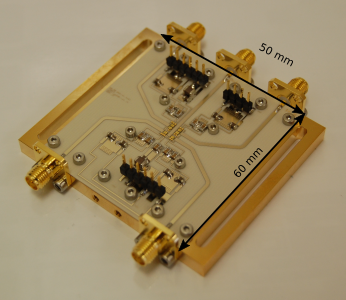
\includegraphics{Demonstrator_publish.png}
	\caption{Built demonstrator}
	\label{fig:Demonstrator}
\end{figure}
To the best of the author's knowledge, the worldwide first realised Riemann Pump in GaN technology is presented in Figure \ref{fig:Demonstrator}.\\

In this work a new concept of digital to analog conversion is investigated yielding an arbitrary waveform generator which can be used in the next generation of mobile communication.
For the development of this waveform generator, a proper concept is researched and simulated, a layout of the test circuit is developed and a first prototype is successfully built and measured.
The presented concept yields a waveform generator which is able to cover the frequency range from DC to \SI{6}{\giga \hertz}, which simulations confirmed.
With the help of this custom digital-to-analog converter, the actual conversion methods of digital to analog conversion are impressively enhanced.
The first Riemann Pump in GaN technology was built to prove the concept of a push-pull stage, providing a multi bit charge pump.
This multi chip solution is chosen to show the feasibility of generating different signals.
Simulations already demonstrates some draw backs and trade offs regarding the power consumption and the bandwidth limitation.
In addition to this, some aspects are mentioned which influenced the signal quality.
In the design and realisation process custom drafts are developed to improve the heat transfer, while guarantee the proper functioning of the test circuit.
Some aspects are considered to reduce parasitic effects and undesired behaviour of the circuit.
After the assembly of the test circuit, different measurement concepts are prepared.
The digital input signal at four input ports required a special control strategy.
In addition, a proper output measurement strategy is described to illustrate the results.
The successful measurement of the built demonstrator finishes the proof of the demonstrated concept.
At last a conclusion sums up the results of the presented work and give an outlook for further improvements and investigations.





%\textbf{Agenda}
%\begin{enumerate}
%	\item literature survey
%	\item adaption of push-pull concept from Maksimovic (Talk at Fraunhofer IAF 06/2015)
%	\item GaN25 \gls{ab:gan} parameter simulation [S-parameter,ON/OFF switching voltage]
%	\item determine load impedance [input of PPA - GaN25 \gls{ab:hemt}
%	\item determine dimension of transistors
%	\item tuning schematic parameter for optimal simulation (special freq?)
%	\item enhancement/extension of 1-bit push-pull to 3-bit push-pull stage
%	\item digital input control voltage
%	\item determine eight slopes of the current sources in schematic 3-bit resolution
%	\item Riemanncode generation with MatLab; minimizing error
%	\item control schematic with theoretical input [Riemanncode]
%\end{enumerate}
%\vspace{1cm}
%\textbf{Problems}
%\begin{enumerate}
%	\item frequency dependent load impedance
%	\item absence of p-type transistor makes it hard to efficiently switch the high side transistor in the Gbps range
%	\item the heat spreading on the chip and substrate is critical
%	\item energy consumption may be very high (mainly switching losses)
%	\item the absence of accurate current sources makes it very hard to get a defined slope for the switching transistors.
%	\item theoretical slope generation very inaccurate
%	\item theoretical slope generation via shorted load  (R = \SI{1}{\ohm})
%	\item \textit {$\rightarrow$ slopes ambiguous}?	
%	\item \textit{$\rightarrow$ riemanncode generation not possible}?                                                                                                                                                                                                                                                                                                                                                                                                                                                                                                                                                                                                                                                                                                                                                                                                                                                                                                                                                                                                                                                                                                                                                                                                                                                                                                                                                                                                                                             
%\end{enumerate}
%\vspace{1cm}
%\textbf{Question}
%\begin{enumerate}
%%	\item mmW band much higher BW,Datarate,Spectrum - why use the old fashioned frequency bands from DC to 6GHz instead of using a couple of GHz?
%%	\begin{itemize}
%%		\item carrier frequencies of modern telecommunication standards are in the range of DC to 6 GHz
%%		\item Signal generation is done for the bandwidth of 0..\SI{6}{\GHz}, after that it could be mixed up to higher frequency bands like \SI{47}{\GHz} to \SI{53}{\GHz}
%%	\end{itemize}
%	\item trade off between BW and losses
%	\begin{itemize}
%		\item higher bandwidth means higher switching speed means higher losses due to the fact that the losses increase linear with the switching speed
%	\item higher frequencies means higher attenuation (e.g. weather condition, like rain)
%	\end{itemize}
%\end{enumerate}

\newpage
\chapter*{Zusammenfassung}

In dieser Arbeit wird ein neus Konzept der Digital-Analog-Umwandlung untersucht, welches ein Signalgenerator ergab, der in der n\"achsten Generation der mobilen Kommunikation verwendet werden k\"onnte.
F\"ur die Entwicklung eines solchen Signalgenerators wurden geeignete Konzepte untersucht und simuliert, ein Schaltungsentwurf entwickelt, ein erster Prototyp aufgebaut, dieser getestet und erfolgreich vermessen.
Das vorgestellte Konzept ergibt einen Funktionsgenerator welcher in der Lage ist Signale im Frequenzbreich von \gls{ab:dc} bis \SI{6}{\giga \hertz} zu generieren, was Simulationen best\"atigten.
Mit Hilfe dieses Digital-Analog Wandlers wurde die Leistungsf\"ahigkeit bisheriger Methoden eindrucksvoll erh\"oht.
Die erste Riemann Pumpe in GaN Technologie wurde aufgebaut um das untersuchte Konzept einer Gegentaktstufe zu best\"atigen, was zu einer Ladungspumpe mit mehreren Bits f\"uhrte.
Um zu zeigen, dass verschiedene Signal generiert werden k\"onnen, wurden mehrere Chips verwendet.
Simulationen zeigten bereits einige Nachteile und Trade-offs was insbesondere den Energieverbauch und die begrenzte Bandbreite angeht.
Ausserdem werden einige Gesichtspunkte erl\"autert, die die Qualit\"at des generierten Signals beeinflussen.
Im Schaltungsentwicklungsablauf werden spezielle Entw\"urfe vorgestellt, die das Problem der W\"armeabfuhr verbessern und gleichzeitig das korrekte Funktionieren der Schaltung sicherstellten.
Einige Aspekte wurden untersucht um parasit\"are Effekte und unerw\"unschtes Verhalten der Schaltung zu reduzieren.
Nachdem die entwickelte Schaltung konkret aufgebaut wurde, wurden verschiedene Messaufbauten vorbereitet.
Das digitale Eingangssignal an den vier Eingangsports ben\"otigte eine spezielle Kontrollstrategie.
Weiterhin ist eine geeignete Strategie beschrieben, die das korrekte Messen am Ausgang erm\"oglichte.
Das erfolgreiche Messen der aufgebauten Testschaltung erbringt den Machbarkeitsnachweis von dem vorgestellten und entwickelten Konzept.
Als letztes fasst die Schlussfolgerung alle wesentlichen Ergebnisse dieser Arbeit zusammen und ein Ausblick f\"ur weitere Entwicklungsm\"oglichkeiten wird gegeben.
}
		

\maketitle	% generates title page, declaration and abstract page
\pagenumbering{roman}	% pages before TOC
\cleardoublepage
\newpage
\thispagestyle{empty}

%\addcontentsline{toc}{chapter}{\numberline{}Themenblatt}

\tableofcontents

\printglossaries
%\printnomenclature

%\listoffigures
%\listoftables

\cleardoublepage
\setcounter{page}{1}

\pagenumbering{arabic}
\chapter{Introduction}
%\textit{A brief summary of the contents of the thesis, including what was done and, in general terms, what was achieved. Two pages maximum}\\
%\textit{Explanation of why you had to do what you did. At the end of this section, you should summarize your most important results in one to two pages, including your best measurement result.}
Mobile communication became a major part of our daily life. 
With the release of the fourth mobile communication standard  \gls{ab:lte} over 70 atomic power plans were required to handle the estimated energy consumption of the world wide mobile communication.
Approximately 70.000 base stations \cite{Bundesnetzagentur2016} are in operation in Germany, which consume an estimated energy of approximately 3 billion \si{\kilo \watt \hour}, based on an estimated power consumption per base station between \SI{2}{\kilo \watt} and \SI{5}{\kilo \watt} \cite{BaseStationEnergy}.
The reason for the huge amount of energy consumption is the immense demand on high data rates.
In our every day life customer applications are dealing with very high data transfer rates.
Today's data rates handle videos in two dimensional resolution, but the next generation have to handle three dimensional high resolution video streams in real time via virtual reality 360$^{\circ}$ cameras.
It will be possible to broadcast a live video stream from a sports event or concert.
In addition to the customer application field, the industry also steadily increase their data volume sent via mobile communication.
It is expected, that the data rate is increasing exponentially up to the year 2020 \cite{BundesnetzagenturfuerElektrizitaet2015}. 
Induced by M2M (machine to machine) communication, real time data transfer is becoming more and more important.
All of the mentioned aspects increase the demand of a new mobile communication standard.
The fifth generation of mobile communication (5G) is expected to be released in the year 2020 \cite{EuropeanCommission2015}.
The vision of the 5G standard is to increase the data rate to \SI{10}{Gbps}, decrease the latency to \SI{1}{\milli \second}, which is equivalent to real time connections and handle more connections than ever before \cite{EuropeanCommission2015}.
But with the new communication standard also new hardware is needed.
The hardware needed, must be able to handle the huge amount of data in real time.
Therefore new concepts were investigated regarding new hardware topologies.
One of the new concepts is presented in this thesis.
It makes use of the principle of full software radio and utilized gallium nitride technology.
This makes it possible to cover the emerging need of a wideband operation, while ensuring a low power consumption.
To reach this wideband operation in a software radio, it is necessary to bring the digital world as close as possible to the analog domain.
Therefore a decent digital-to-analog converter is needed which is investigated in this thesis, named Riemann Pump.
The progress of the development of such a digital-to-analog converter, contains several steps.
First of all a literature survey is performed.
This survey yields some basic concepts for the Riemann Pump, which were adapted to design a test circuit in \gls{ab:gan} technology. 
For the \gls{ab:gan} technology different concepts are investigated and evaluated.
After the development of a concept, detailed simulations are performed to get an insight in the properties of the Riemann Pump.
The simulations are run with transistors modelled at the \gls{ab:iaf} \cite{Model}.
Afterwards strategies are presented which exhibit some important aspect for the assembly of the test circuit.
The measurement results are presented in chapter \ref{ch:measurement}.
The successful measurement required a proper input control and output measurement strategy, which are demonstrated.
The assembled multi bit demonstrator is measured for the first time, since no results were published regarding a Riemann Pump in \gls{ab:gan} technology.
The measurement results of the built prototype are presented and confirm the proof of concept.


%Sendeleistung der Basisstation betraegt 20W. Elektronische Komponenten brauchen aber mehrere tausend Watt (kW) um die Informationen an den Empfaenger zu senden. PA am wichtigsten, hohe leistung, geringe Leistungsaufnahme, hohe frequenz. mehr als 70.000 Basisstationen deutschlandweit, Energieverbrauch/Jahr: 2 Mrd kWh entspricht der jaehrlich eingespeisten Energie eines kleinen Kohlekraftwerks. Energiebedarf weltweit werden etwa 70 Kernkraftwerke noetig. Mobilfunknutzer steigt: 2020 4.6 Mrd Nutzer, 2020 1800 Billarden Bytes, technisch energieeffiziente loesungen noetig ohne umwelt zu belasten. 5G bis 2020. 1 Mrd bit/s 10mal soviel wie LTE. Extrem schnelle und energieeffiziente power amplifier. Avlanche breakdown! UMTS Basisstation: 20km, LTE mehr Daten weniger Reichweite, hoehere Frequenz: 5km,Reichweite muss in der naechsten Generation auch erhalten bleiben, also viel Leistung auf noch hoeheren Frequenzen. Silizium schafft die Leistung nicht, das Silizium wuerde viel zu heiss, deswegen III-V Verbindungshalbleiter. 3000 Watt Energieaufnahme um mit fuenf antennen jeweils 20 Watt im Umkreis von 20km fuer 600 Telefonate gleichzeitig zu verteilen. Filme, Musik, Stream -> Datenrate und zwar 10 bis 100-fach hoehere Datenrate als LTE. 100 Milliarden Geraete sollen gleichzeitig ansprechbar sein WELTWEIT (Computer,PDA, Auto, Smartphone etc.). Latenzzeiten von unter 1 ms!! Fast Echtzeit, Maschinenkommunikation !! Maschinen sind sehr empfindlich und muessen zu jedem Zeitpunkt wissen wo sie stehen. Energieverbrauch soll um ein tausendstel pro bit gesenkt werden. (insgesamt soll der stromverbrauch um 90 prozent verringert werden) GaAs wird vollstaendig verschwinden, sowohl mobil als auch basisstationen werden auf \gls{ab:gan} umruesten muessen. Neue Geraete werden notwendig, 5G wird nicht kompatibel sein mit den alten Standards. 
\chapter{State of the art, Research and Development of 5G mobile communication}
Research and development of the next generation of mobile communication. Mobile Congress 2016 in Barcelona, Huawei \& Telekom present a first data link in 73 GHz with a few Gbps.\\
First attempts on a digital to analog converter for the frequency range based on the concept of a charge pump, were designed by french people Veyrac et. al\\
Mark Zuckerberg hold a speech about fifth generation of mobile communication. The goal is to provide and deliver internet to everyone in every country.  
\chapter{Fundamentals-Theory for this approach to reach 5G}
In the following some fundamentals are described shortly.
\section{Concept of Software-defined radio}
The concept of software-defined radio is adapted to deal with the old problems of mobile communication. The idea is to bring the digital domain as close as possible to the RFFE. The reason is digital filtering, data processing is more efficient, easier, less complex, has less cost, and so on. The main problem of this approach is the energy consumption based on an inefficient ADC/DAC. However the concept is very helpful for future designs of an digital front end. The Software-defined radio has the advantage, that it is adaptiv for future software changes. the hardware is still the same, only the firmware has to be upgraded. broad spectrum of signal can be received with this architecture. from nearly DC to 2 GHz. For future mobile communication standards, the frequency range has to deal with frequencies beyond 2 GHz up to 6 GHz. Nowadays IEEE802.11ac standard is located at 5GHz. Based on this concept a digital-analog converter is designed to deal with a higher bandwith than other devices nowadays. The DAC is used in the transmission path of the design.
\section{An approach to reach the desired high speed for the digital-to-analog converter: The Riemann Pump}
\subsection{Idea of the Riemann Pump}
The Riemann Pump, named after the mathematician Riemann, who founded the Riemann Integral, is a special charge pump. A charge pump as the name suggests pumps electrons into a capacitve load. Across the load capacitance a voltage is created. By adjusting the switches for up or down the voltage can be adjusted, as seen in Fig. \ref{ChargePump}. 

\begin{figure}[ht]
	\centering
  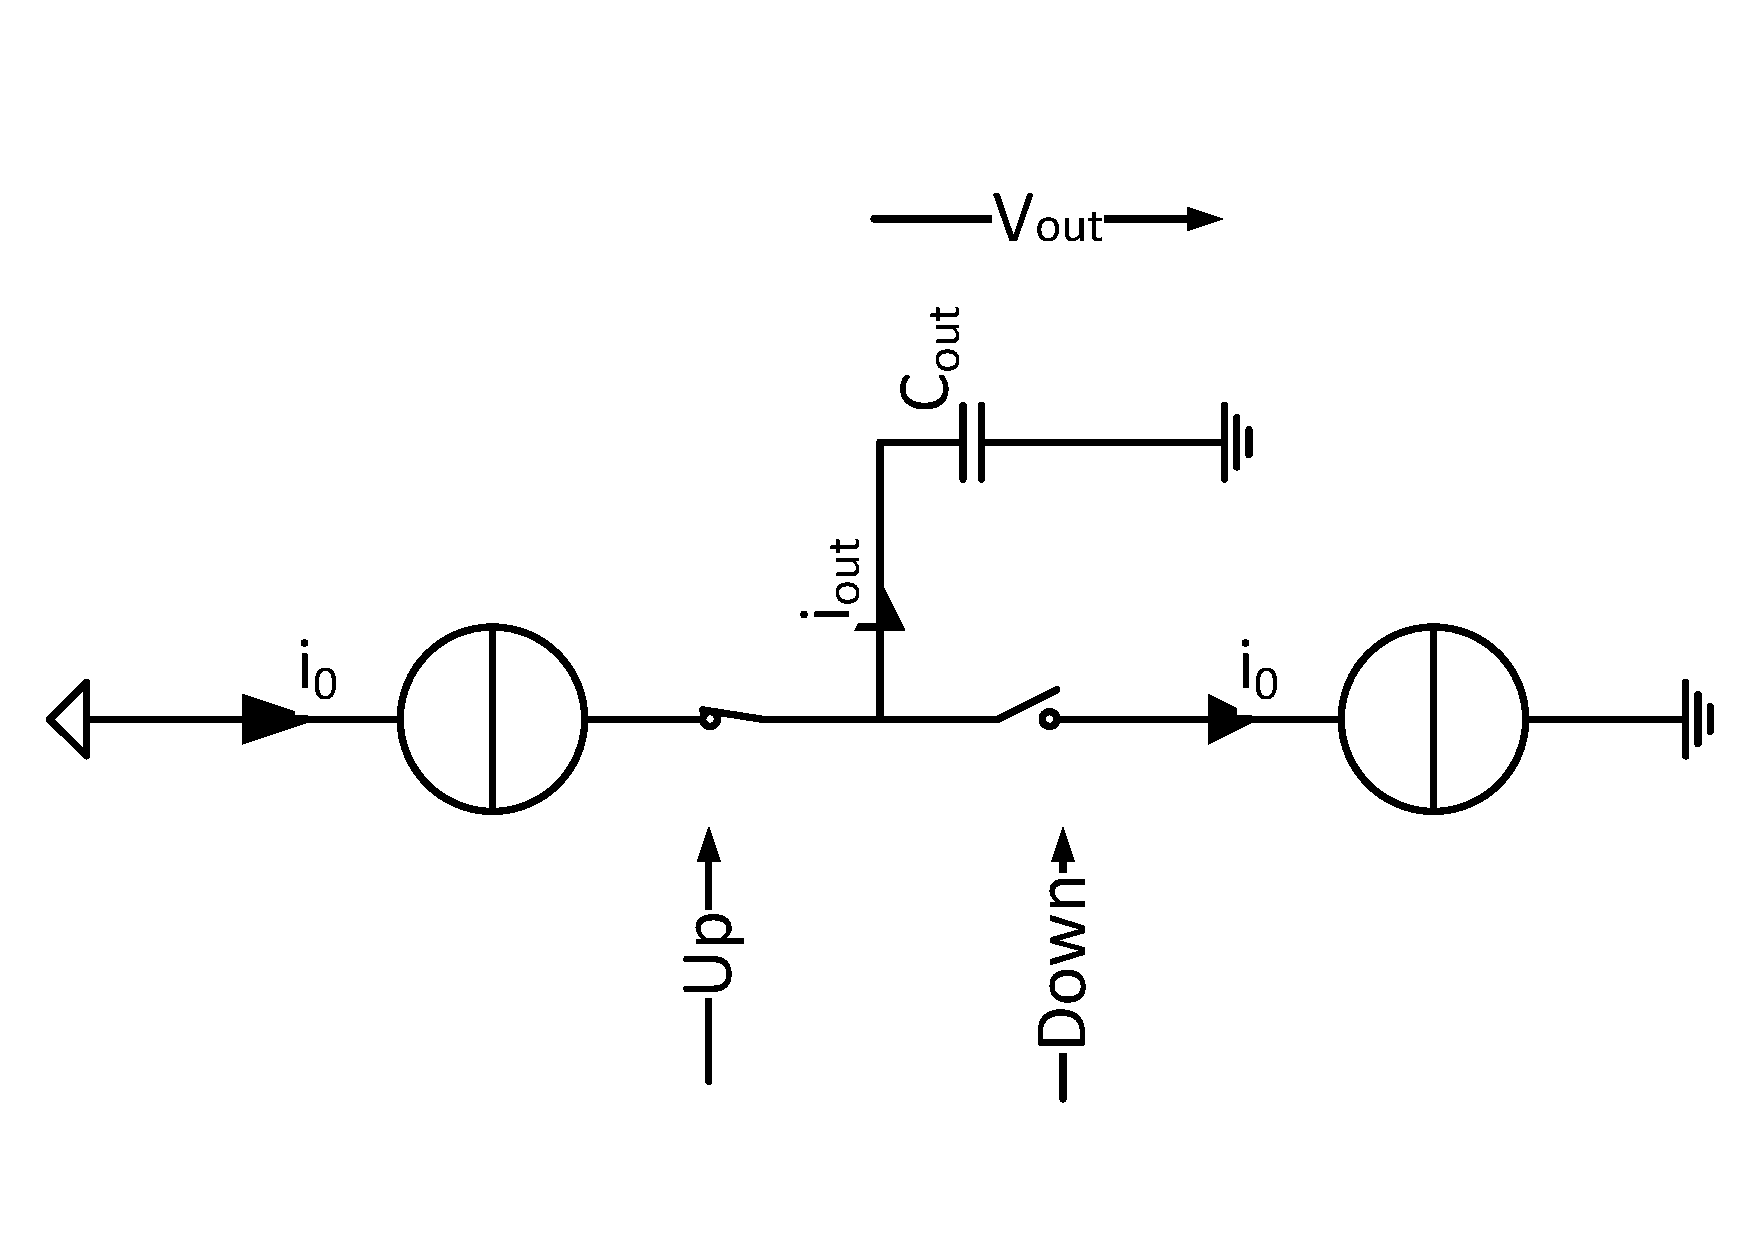
\includegraphics[width=0.5\textwidth, angle = 270]{ChargePump.pdf}
	\caption{scheme of a charge pump; works like a Riemann Pump with one-bit resolution}
	\label{ChargePump}
\end{figure}

The Riemann Pump is a digital-to-analog converter based on the concept of a charge pump. A few charge pumps with different sized sources in parallel shows the concept of this fast digital to analog converter. With the ability to control the switches really fast, because of the use of GaN25 technology, which have a high transition frequency, a high bandwidth is reached.

\begin{figure}[ht]
	\centering
  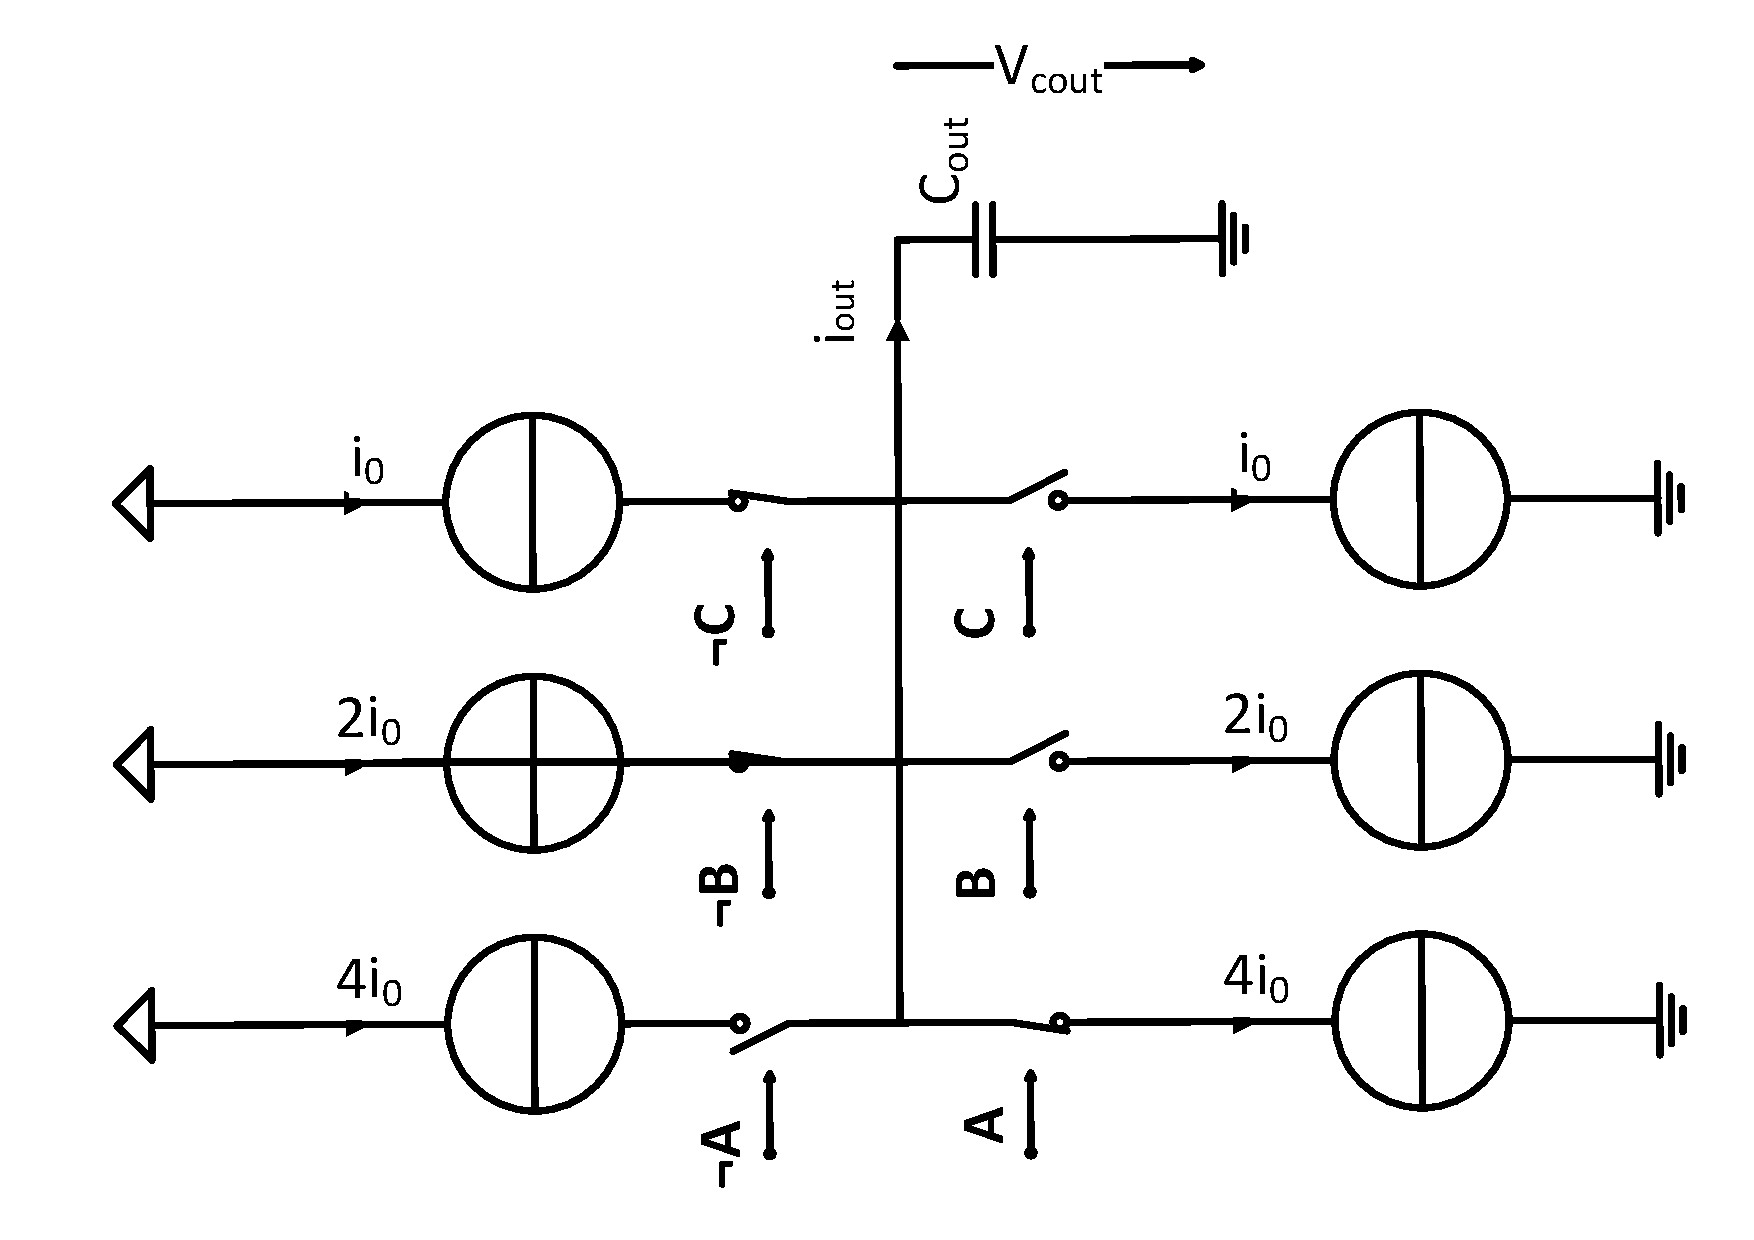
\includegraphics[width=0.5\textwidth, angle = 270]{RP_concept.pdf}
	\caption{Concept of the Riemann Pump with three-bit resolution}
	\label{RiemannPumpConcept}
\end{figure}

 The working principle is to
integrate a current into a capacitive load, this integration is based on Riemann Integral, where the name come from. This integration converts the current into a voltage. This output voltage can be applied to the input of a power amp and then to the antenna to propagate it. The current, which charges the capacitive input of the power amp, is controlled by a digital code. A fixed set of slopes, represents the different current sources. A desired signal in the time-domain is generated with MatLab. This signal can consist of many different signals (different carriers and modulation types). This signal is sampled with the given set of slopes. The minimization of the error leads to the Riemann Code. With this Riemann Code (digital) the driver circuit is controlled. This leads to an analog signal formed by the digital input signal. The signal to noise ratio is calculated in equation \ref{eq:SNR_RiemannPumpConversion}. Quantization noise model {reference: analog}
\begin{equation}
	\text{SNR } [\si{\dB}] = 6.02N + 9.03r - 7.78 + 10\log_{10}(1 - \frac{1}{2}^{N-1} + \frac{1}{2}^{2N})
	\label{eq:SNR_RiemannPumpConversion}
\end{equation}
\subsection{implementation of the idea - realisation}
The first approach of designing a Riemann Pump was with a concept of a Push-Pull stage. This push-pull stage should charge a capacitive load at the output, which is the same as a normal charge pump. Push-pull stages complementary switch a high- and lowside transistor as in a charge pump. This was one possible approach. Concept of Maksimovic. 
\subsection{challenges to review - problems}
Same realisation problems, difficulties: Problem of BANDWIDTH, Vpp of control signal (5V pp for GaN transistors), high side driver, no complementary transistors available in III-V technology, low loss driver, high speed driver, digital control driver, too high energy consumption (stability???)
\chapter{Riemann Pump circuit design}
\label{ch:design}
% \textit{Description of the approach you have taken to solve the scientific or technical problem which you were posed. Outline the design, the methodology and overall structure of your experimental approach}\\
The goal was to design an arbitrary waveform generator for a signal bandwidth of \SI{6}{\giga \hertz}.
For the implementation in a base station, the most promising technology was \gls{ab:gan}.
\gls{ab:gan} \glspl{ab:hemt} were used for the high speed switches, which served as voltage controlled current sources.
Based on the chosen technology a suitable push-pull concept were found \cite{MaksimovicPaper} to show the feasibility of the concept.
The attention was rather drawn to proof the concept than to optimize for energy consumption or efficiency.
In the design process a suitable load impedance and the right dimension of the used components had to be found.

\section{Approach and implementation of the Riemann Pump}
As stated in chapter \ref{IdeaRiemannPump} the circuit needed high speed switches, which were capable to drive power.
The absence of a p-type transistor in \gls{ab:gan} technology made it challenging to find a suitable concept to realize the push-pull stage.
Since the n-type \glspl{ab:hemt} needed a negative gate source voltage \gls{sy:vgs}, the high side switch could not be implemented without a driver circuit.
The source contact of the high side switch, realized by a n-type \gls{ab:gan} \gls{ab:hemt}, was connected to the output of the test circuit.
Since the potential at the output was not constant, this high side switch needed a driver circuit.
A suitable driver circuit was found in \cite{MaksimovicPaper}, where the principle of a push-pull stage for power applications is described.
The benefit of the integrated driver circuit was the improved efficiency of switching.
The transistor switching speed was determined by the dimension of the driver circuit.
If the switching speed was increased, the gate driving current \gls{sy:IG} has to be increased to switch the transistors.\\
One possible approach to design a Riemann Pump is shown in Fig. \ref{fig:SchematicRiemannPump}.

\begin{figure}[ht]
	\centering
  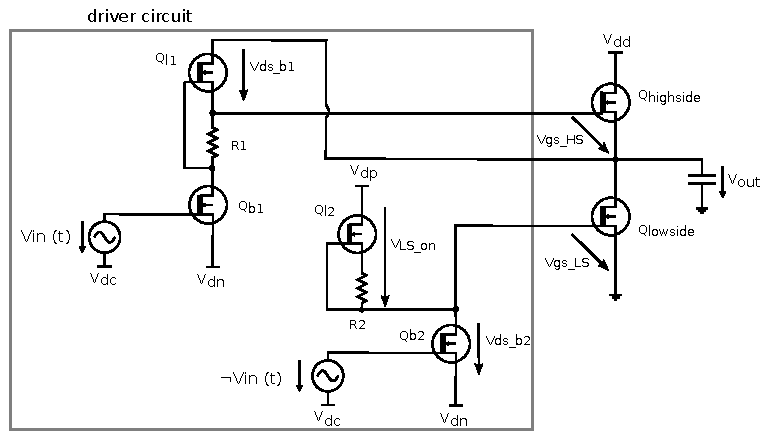
\includegraphics{Schematic_RP_concept2.pdf}
	\caption{Schematic of a push-pull stage with corresponding driver circuit}
	\label{fig:SchematicRiemannPump}
\end{figure}

On the left side, as marked, is the driver circuit which was needed to switch the high side transistor without dissipating a huge amount of power.
As the timing is crucial for the switching process, the driver concept was implemented for the low side switch too.
The schematic shows the first approach for realizing a Riemann Pump in \gls{ab:gan} technology.
The next step was the identification and calculation of a proper output capacitance, since it represented the input of a linear power amplifier where the desired signal is synthesized.
 
\section{Identification of the load impedance} % VERBESSERN!
The signal is generated at the input stage of a linear power amplifier, as described in chapter \ref{ch:fundamentals}.
This output stage is modelled with a \gls{ab:gan} \gls{ab:hemt} with a gate length of \SI{0.25}{\micro \meter}.
Considering a \SI{20}{\watt} power amplifier for transmission purposes, led to a \gls{ab:gan} \gls{ab:hemt} with a total gate periphery of \SI{4}{\milli \metre}, based on an approximation for the power density of \SI[per-mode=fraction]{5}{\watt\per\milli\metre} gate periphery  \cite{Maroldt2010}, \cite{GaNBook}.
Simulations confirmed this approximation as an output power density of \SI[per-mode=fraction]{5.6}{\watt\per\milli\metre} at $V_{DS} = 25 V$ was measured.
This transistor model \gls{ab:hemt} (IAF\_GE\_MSL\_ A204/IAF\_GaN25\_HEMT\_CS\_LS\_SHfull) used in \gls{ab:ads} were modelled at the \gls{ab:iaf}\cite{model} and is based on a state-space approach. 
For simulation purposes four transistors were modelled in parallel, each with 8 finger and \SI{125}{\micro \metre} gate width to reach the required gate periphery.
The simulated power amplifier is biased with respect to the maximum \gls{ab:mag}, which led to a bias of $V_{GS} = -1.5 V$ at $V_{DS} = 25 V$.
After the determination of the bias point, a S-parameter simulation yielded the input reactance of the power amplifier.
It is to note that four power transistors were simulated for the purpose of a power amplifier, hence this did not respect the broadband application since it was no broadband amplifier.
Since the capacitive behaviour of the load impedance is of interest, the real part is for now neglected.
The input reactance $X_c$ is defined as:
\begin{equation}
	X_c = -\frac{1}{\omega C},
\end{equation}
\label{eq:reactance}
and is plotted in Figure \ref{fig:inputReactance} over the frequency range from nearly \gls{ab:dc} to \SI{6}{\giga \hertz} in a logarithmic scale.

\begin{figure}[ht]
	\centering
  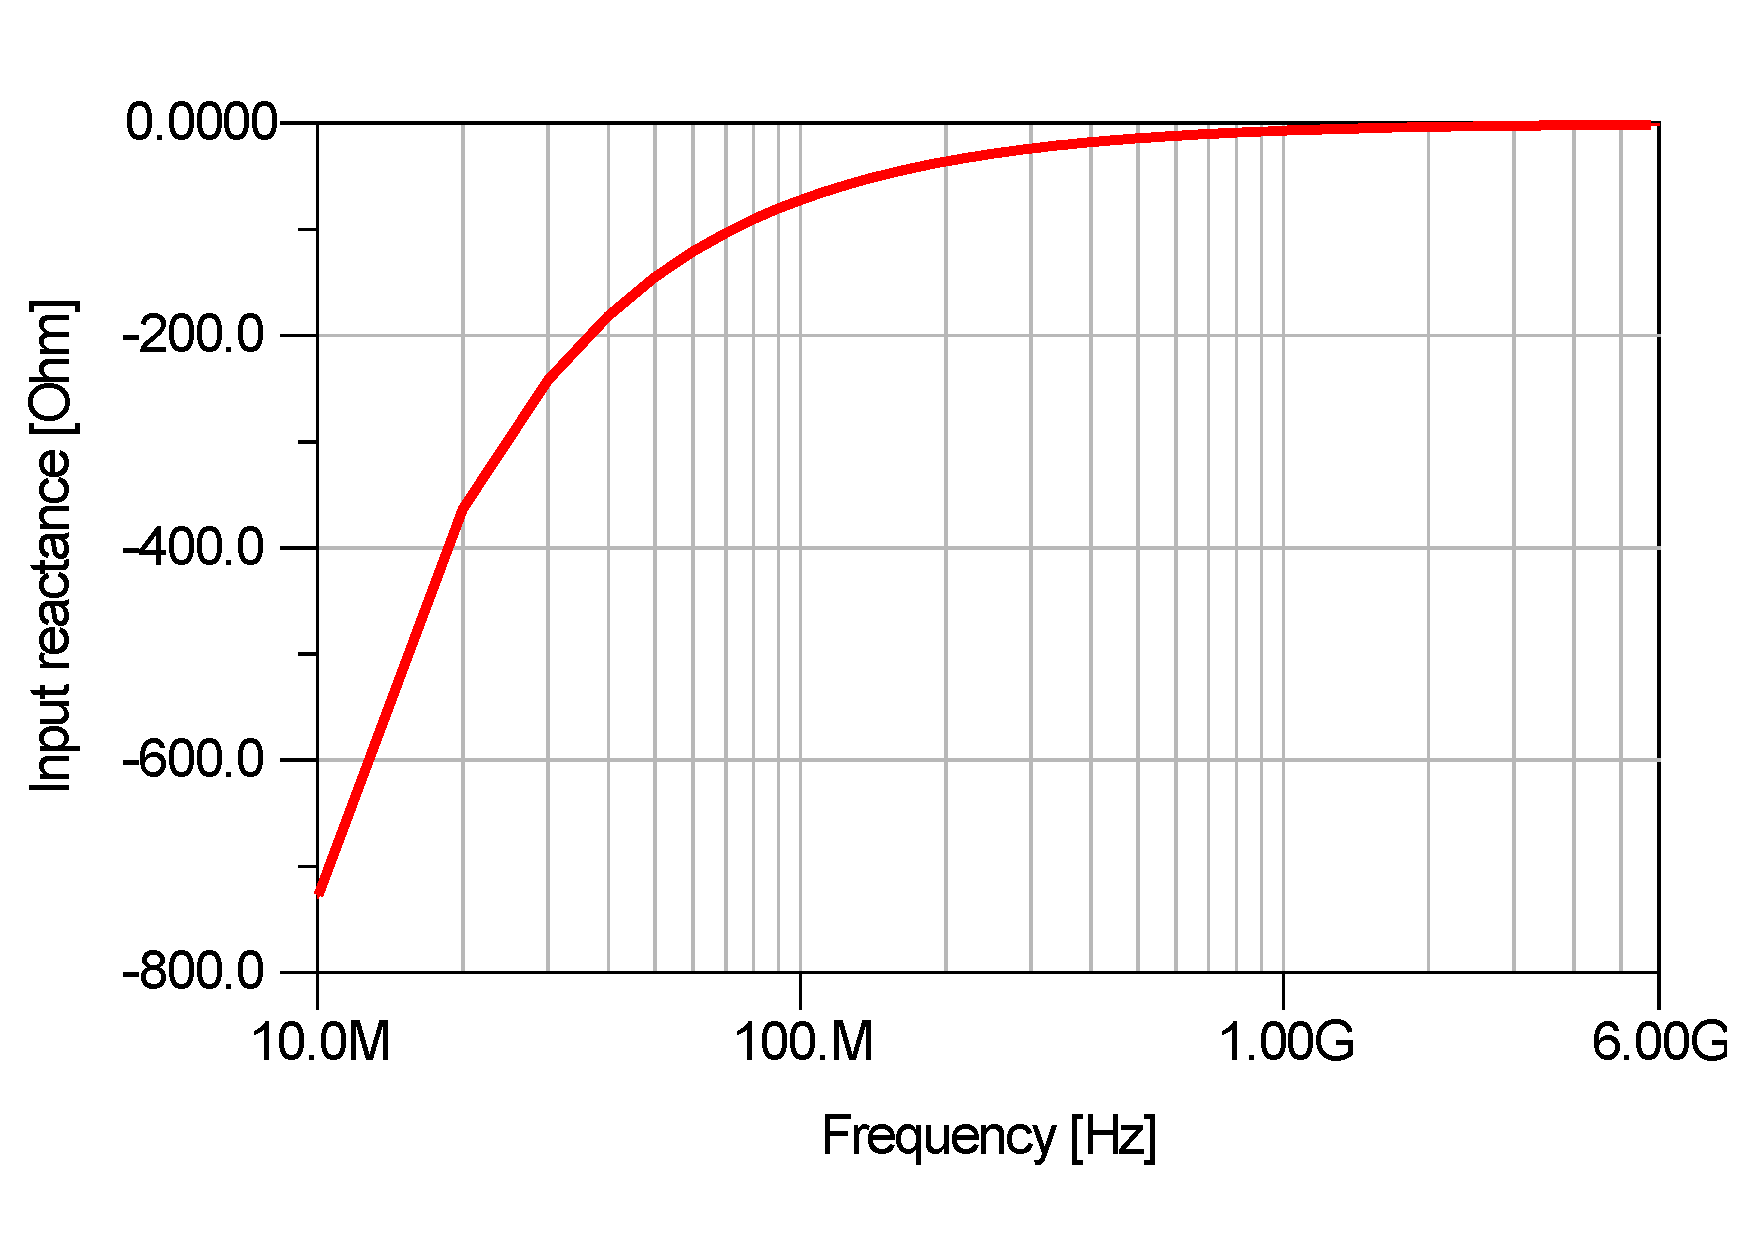
\includegraphics[width=.75\textwidth]{inputReactance.pdf}
	\caption{load reactance}
	\label{fig:inputReactance}
\end{figure}

As the reactance of the simulated power amplifier is nearly constant for the frequency of \SI{1}{\giga \hertz} and beyond, this showed the impact of parasitic effects.
For frequencies in the \si{\giga \hertz} range the parasitic inductances reduced the reactance.
Interpreting the minus sign only for the phase delay, since it is capacitive, the absolute value of the reactance decreases exponentially with the frequency up to approximately \SI{1}{\giga \hertz}.
Solving the equations \ref{eq:reactance} absolute value for the capacitance yielded:

\begin{equation}
	C = \frac{1}{\omega X_c},
\end{equation}
which is illustrated in Figure \ref{fig:inputCap_log}.
As a large signal model was used for the simulation, the inductive part of the input impedance got bigger.
This effect is seen in \ref{fig:inputCap_log} for frequencies beyond \SI{1}{\giga \hertz}.
%The frequency dispersion effect on the input capacitance of the \gls{ab:gan} \gls{ab:hemt}
\begin{figure}[ht]
	\centering
  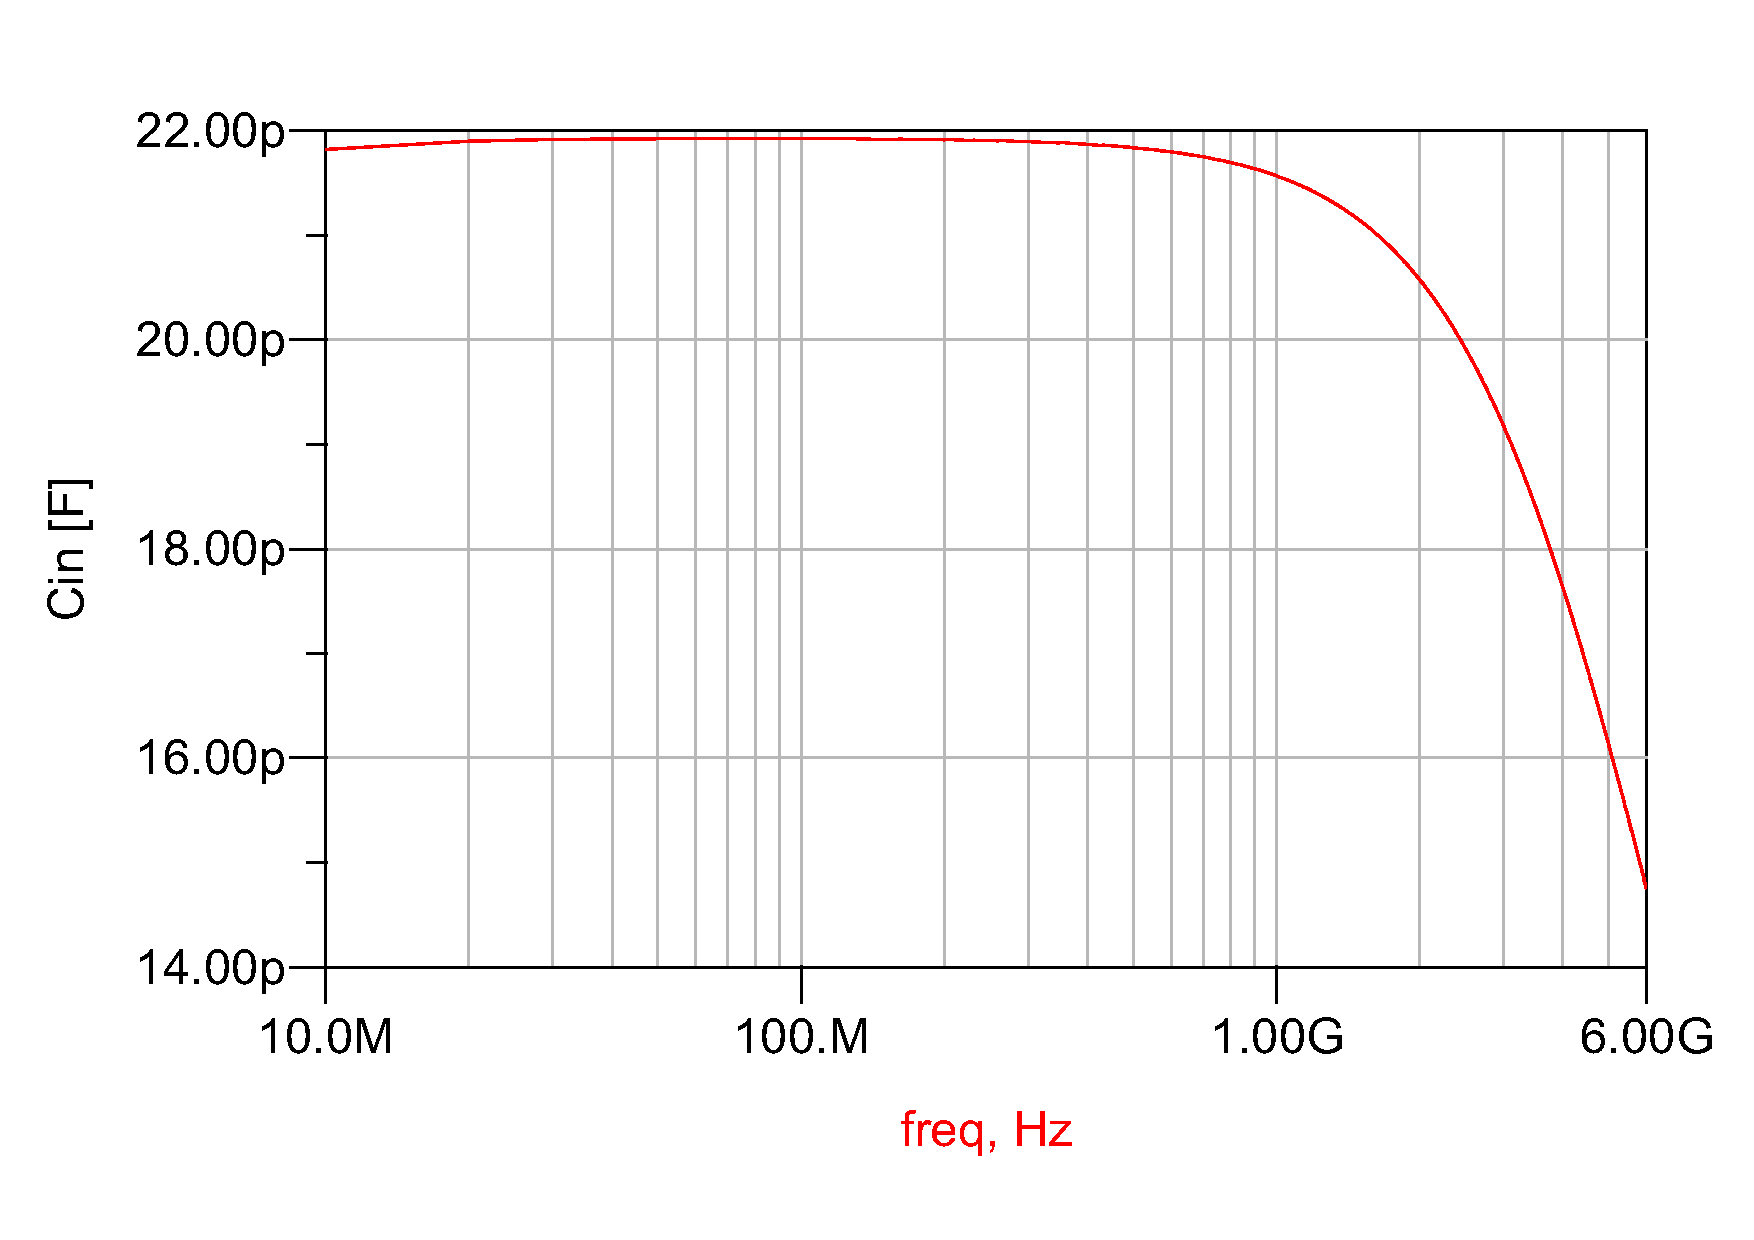
\includegraphics[width=.75\textwidth]{inputCap_log.pdf}
	\caption{load capacitance log}
	\label{fig:inputCap_log}
\end{figure}

Nevertheless the complex input impedance yielded a capacitive behaviour with a value of nearly \SI{22}{\pico \farad}, which was used for further investigations.
The simulated transistor model was specified as a large signal model, as seen in Figure \ref{fig:inputCap_log} for frequencies beyond \SI{1}{\giga \hertz}.
Frequency dispersion and other parasitic effects appeared, which could not be investigated due to the limited scope of this thesis.

%
%Since the input capacitance can be assumed as 
%\begin{equation}
%	C = \epsilon_r \frac{A}{d},
%\end{equation}
%
%it follows that
%\begin{equation}
%	C \propto \epsilon_r 
%\end{equation}
%
%and therefore for high frequencies, the capacitance is decreasing due to decreasing dielectric constant for \gls{ab:gan} \cite{GaNBook},p.7. % pdf page 33
%Degrading capacitance due to non-linearities.

%Due to the non-linearity of the transistor model \cite{vitanovnon}
%The frequency dependent input impedance [\textbf{REFERENCE}], which corresponds to the load impedance of the designed Riemann pump circuit, is determined by S-parameter simulations.
% small signal is not considered, since only the curent integration is important

%%% 27.04.2016 01:34 Uhr
\section{Dimension of the used components}
An input capacitance of nearly \SI{22}{\pico \farad} was found for the output linear power amplifier stage.
Based on this calculation a proper test circuit was investigated.
To avoid immediate clipping of the signal at the output, the transistor dimension had to fit, since an oversized transistor would fully charge the capacitance and the signal would be clipped.
Hence a transistor dimension was chosen which allowed to synthesize a decent signal.
To synthesize a sine wave for the frequency of \SI{6}{\giga \hertz} with a voltage swing of $V_{swing} = 4V$, the two greatest slopes were chosen.
In the presented concept the resolution is three bit, hence eight different current slopes could be generated.
The sequence of the relative slopes $7 i_0$ and $5 i_0$ synthesize the rising edge of the sine wave.
With this relative slopes and an oversampling ratio of four at the frequency of \SI{6}{\giga \hertz}, led to a sampling time $\Delta t$ of \SI{20.83}{\pico \second}, since the sampling frequency is eight times the signal bandwidth.

The current-voltage relation for the capacitor
\begin{equation}
	I = C \frac{d U}{d t},
\end{equation}
is used to determine the reference current $i_0$.

A voltage swing of $V_{swing} = 4V$ is equal to an amplitude of $\hat{v} = 2V$.
The oversampling of four yielded, that the sine signal is sampled by eight points.
Hence the rising edge consisted of two sampling points.
The first sampling point with the relative slope of 7 and the second of 5, respectively.
Integrating the current for two different samples yield:

\begin{equation}
\int_{\Delta t} 7 i_0 d\tau + \int_{\Delta t} 5 i_0 d \tau = C*U,
\end{equation}

and solving for $i_0$ resulted in:

\begin{equation}
i_0 = \frac{U*C}{12*\Delta t}.
\end{equation}

For the assumption to reach nearly a voltage of $\hat{v} = 2V$ for two sampling intervals ($2 \Delta t$) and the capacitance of \SI{20}{\pico \farad} it resulted a reference current of $i_0 = \SI{160}{\milli \ampere}$.
%The dimension of the switching transistors, which represent a voltage controlled current source, determines the maximum current flowing.
%This current source is controlled by a digital signal which determines it to be fully open or to be closed, as a switch.
As simulations showed, a reference current of $\SI{151}{\milli \ampere}$ could be established with a dimension of the voltage controlled current source, high side switch, of UGW = 100 \si{\micro \meter} and gate finger number of eight.
Hence the gate periphery for the reference current source is \SI{800}{\micro \meter}.
To ensure proper switching the driver circuit dimension had to be optimized.
Since the driver circuit worked as a current source, the dimension of the transistors and resistors were tuned to achieve a proper current to switch the power transistors fast and efficient.
The dimension of the driver transistors were approximately a quarter of the power transistors, the switching high and low side transistor.
The resistor values were achieved by tuning with respect to power consumption.
Further details on the driver circuit and its properties are stated in \cite{MaksimovicPaper}.
The schematic is designed with \gls{ab:ads}, see Appendix \ref{app:schematic}.
As the dimension of the power stage scales with the factor of two so the driver circuit dimension do.

\section{Circuit design summary}
As no complementary transistors were available in III-V technology a proper driver circuit had to be investigated.
Further the speed of the switches was crucial as a broadband signal should be synthesized, which led to the implementation of a known concept \cite{MaksimovicPaper} for the driver circuit.
A low loss, high speed, digital controlled driver circuit was implemented.
Using this concept had the advantage of verification and validation.
It was difficult to determine the reference current since the switching is not ideal, a leakage current through the driver circuit occurs and the current had to be probed in the transient state.
The problem of not perfect switching is, that the channel is opened and closed slowly in comparison to an ideal switch.
This increase the current with the increase of charges flowing to the transistors gate.
Therefore the reference current is time-averaged.
The circuit design and simulation combines the dc state with the rf state.
For a dc simulation the current through a capacitor is zero.
Further the loaded voltage controlled current source was not defined for the given output load.
The dimension of the used components determined the resulting voltage step.
A typical (draw-back) contradiction was a small transistor dimension could synthesize signals to a very low signal frequency while a bigger one would fully charge the output capacitor which will clip the output signal, for a given oversampling ratio.
Because then the sampling time is fixed.
If the transistor dimension is chosen to be bigger, the higher signal frequency could be synthesized with a decent voltage swing but the low signal frequencies would turn into a rectangular shape. 
This problem restricted the signal bandwidth to be smaller than from \gls{ab:dc} to \SI{6}{\GHz}.

%  The components used, were optimized with respect to the signal integrity. 
%  The dimension of the used components were tuned while simulation to get the desired output signal.
%In contrast to the small one a bigger one will be able to synthesize a signal at 6GHz due to the fact that the amplitude would be moderate.

%The smallest current is determined by the dimension of the transistor, which drives into saturation. 
%The smallest saturated current is determined by the push-pull transistor geometry, here: 532 mA.}
\chapter{Circuit simulations for generating various waveform signals}
Circuit simulations were run to validate the behaviour of the conceptual design and to present the trade offs.
A harmonic balance simulation was used to investigate the concepts of chapter \ref{ch:design}, as it presented a steady state solution neglecting the transient state.
This frequency domain simulation was run with the tool \gls{ab:ads} to present the solution for the nonlinear behaviour of the test circuit.
In a first step the generation of various analog output signals were investigated.
Three basic signal waveforms were synthesized to show the ability of generating different signals.
Afterwards the designed test circuit of chapter \ref{ch:design} was tested with respect to stability and its energy consumption.
As the realized circuit differed a bit from the presented test circuit in chapter \ref{ch:design}, another simulation was run to get an impression what to expect for the measurement.
The presented simulations were run with the schematic shown in appendix \ref{app:schematic}, except for the simulation of the built demonstrator in chapter \ref{ch:ProofOfConceptWithExistingComponents}.

\section{Generating various analog signals with digital input control}
Generating analog signals from a digital input signal was the aim of the presented work.
The designed custom \gls{ab:dac}, the Riemann Pump, should be able to synthesize various waveform signals at the output.
Simulation results were presented in the time domain to validate the integrity of the desired signal.
In the system design a pre processor is used to compute the Riemann Code with a specific algorithm.
For simulation purposes the digital Riemann Code was computed manually, as seen for example in Figure \ref{fig:RiemannCodeGenerationSineWave}.
A prerequisite for the design process was a resolution of the \gls{ab:dac} of three bits.
Another prerequisite was an \gls{ab:osr} of four, as discussed in chapter \ref{ch:fundamentals}.
The presented simulations of the digital-to-analog conversion were run to proof the concept of the designed test circuit.
 
\subsection{Sine wave generation in the time domain}
As known from basic signal processing, the sine wave for continuous time is the elementary signal and therefore synthesized first. 
For the generation of this sine wave a corresponding Riemann Code was required which will be converted to the desired sine wave.\\
This Riemann Code was generated by hand via an approximation of a sine wave with a sequence of eight different slopes.
Eight different slopes represented the three bit resolution while the sequence of eight sampling points represented the \gls{ab:osr} of four. 
Figure \ref{fig:RiemannCodeGenerationSineWave} illustrates this approximation to get the corresponding Riemann Code.

%\begin{figure}[htb!]
%   \centering
%   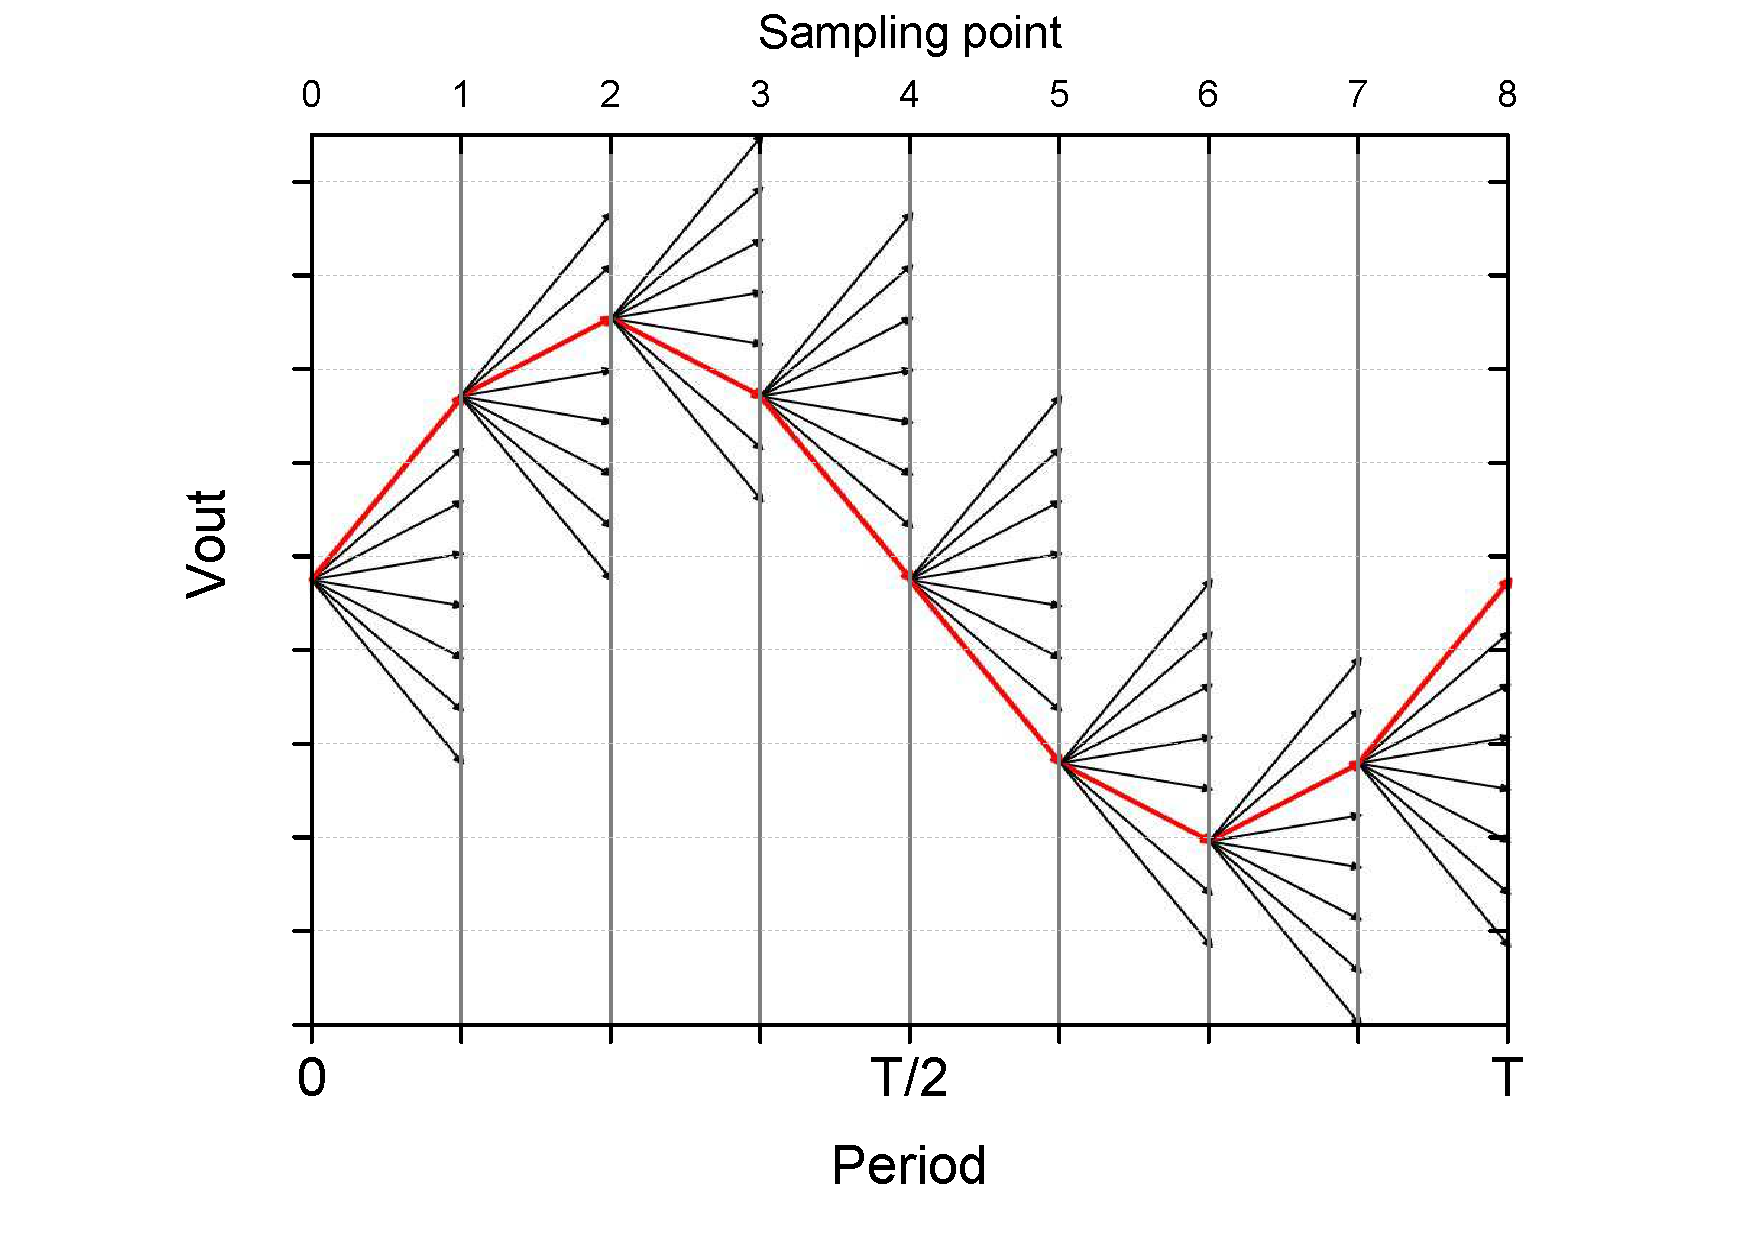
\includegraphics[width=0.75\textwidth]{RiemannCodeGeneration.pdf}
%   \caption{One possible approximation of sine wave generation to get the Riemann Code}
%   \label{fig:RiemannCodeGenerationSineWave}
%\end{figure}

%To validate the feasibility of the presented concept, a digital input control code is required.
%To get this code an approximation by hand is done since no algorithm exists which can compute this.

\begin{figure}[htb!]
   \centering 
   \input{graphics/simulation/RiemannCodeGenerationSineWave73_latest.pdf_tex}
   \caption{One possible approximation of a sine wave generation to get the Riemann Code}
   \label{fig:RiemannCodeGenerationSineWave}
\end{figure}


The sequence of chosen slopes, referred to $i_0$ values, is:
\begin{equation}
 +7\hspace{.3cm} +3\hspace{.3cm} -3\hspace{.3cm} -7\hspace{.3cm} -7\hspace{.3cm} -3\hspace{.3cm} +3\hspace{.3cm} +7,
 \end{equation} 
which represents the following encryption:
\begin{equation}
000\hspace{.3cm} 010\hspace{.3cm} 101\hspace{.3cm} 111\hspace{.3cm} 111\hspace{.3cm} 101\hspace{.3cm} 010\hspace{.3cm} 000,
\label{eq:RiemannCodeSineWave} 
\end{equation}

based on the encryption table in Figure \ref{fig:SlopesAndTable}, chapter \ref{ch:fundamentals}.
The generated Riemann Code consists of eight triplets, where each triplet represents the three bit resolution.
The quantity of digits in each set, here triplet, increases with the number of bits used for the resolution.
The number of triplets represents the number of sampling points, corresponding to the \gls{ab:osr}.
This particular generated Riemann Code in equation \ref{eq:RiemannCodeSineWave} was used to synthesize sine waves in the frequency range between \SI{500}{\MHz} and \SI{6}{\GHz}, as shown in Figure \ref{fig:7SignalsSameSlopeInOnePlot}.

%\begin{figure}[htb!]
%   \centering 
%   \input{graphics/simulation/Vout_sine_SigBWdifferent_SameSlope_73_TwoPeriods.pdf}
%   \caption{Synthesized signals with demonstrated Riemann Code for the frequency range of \SI{0.5}{\GHz} to \SI{6}{\GHz}}
%   \label{fig:7SignalsSameSlopeInOnePlot}
%\end{figure}

\begin{figure}[htb!] %% Add sampling points at the top !!
   \centering
   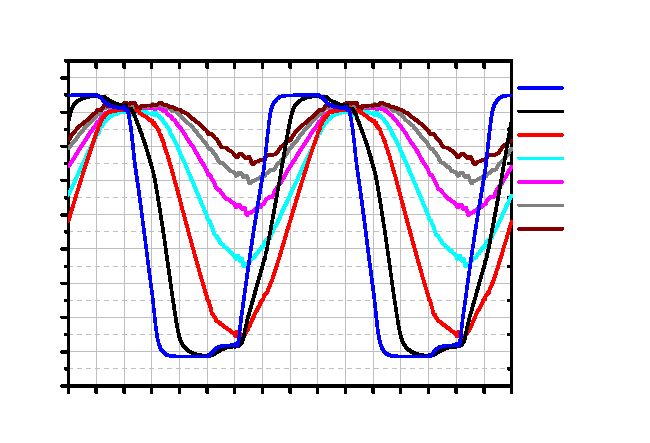
\includegraphics[width=0.75\textwidth]{Vout_sine_SigBWdifferent_SameSlope_73_TwoPeriods.pdf}
   \caption{Synthesized signals with demonstrated Riemann Code for the frequency range of \SI{0.5}{\GHz} to \SI{6}{\GHz}}
   \label{fig:7SignalsSameSlopeInOnePlot}
\end{figure}


The amplitude of seven signals with different frequencies are shown over their period while at the top the number of sampling points is shown.
This representation is chosen to compare the signal integrity of different frequencies.
The shape from most of the plotted functions fit fairly to a theoretical sine wave.
As the sampling interval differs for different frequencies, the amplitudes of the signals also differed.
The maximum reachable amplitude was the positive supply voltage, here set to \SI{15}{\volt}, while the lower bound was \SI{0}{\volt}. 
Once the amplitude reached the supply voltage, the signal wave form is clipped due to a fully charged output capacitor.
This undesired effect transformed the sine wave into a rectangular shaped signal form, as seen for the blue and black curve.
Therefore a bandwidth limitation is introduced.\\
Figure \ref{fig:7SignalsSameSlopeInOnePlot} highlights a limitation of the designed circuit as the blue curve turns into a rectangular signal form.\\

\begin{figure}[htb!] %% Add sampling points at the top !!
   \centering
   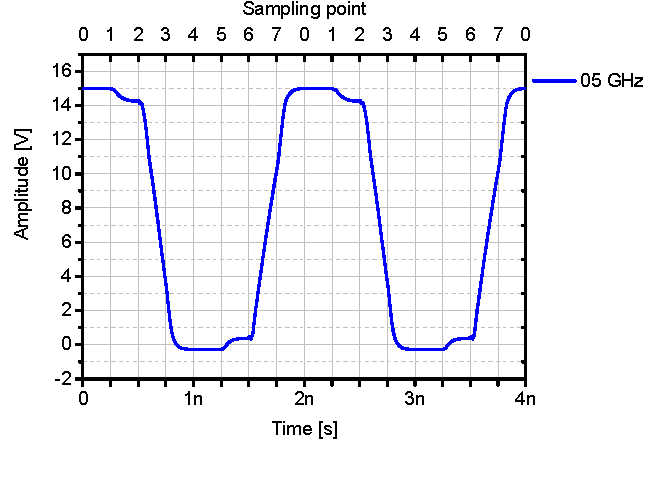
\includegraphics[width=0.75\textwidth]{Vout_sine_SigBW_05GHz_3bit_long.pdf}
   \caption{Synthesized sine wave for frequency of 0.5GHz}
   \label{fig:SineWave05GHz}
\end{figure}


Below the frequency of \SI{1}{\GHz} the desired shape of a sine wave was transformed to a rectangular  form due to the long sampling time.
In addition to the unwanted rectangular form another distortion occurred, depicted in the blue signal for the sampling interval 1 to 2 and 5 to 6.
An unsymmetrical switching process, the finite rise time of the provided current and the not perfectly defined current sources were three factors to mention. %, as the gate of the switching transistor had to be charged 
Furthermore a leakage current were induced by the commutation time of the switching process.
This distortion was mainly observed for low frequencies when the output capacitance was fully charged and discharged.
In the higher frequency range this did not effect the integrity very much.
As already mentioned in the design process, the circuit was designed to fulfil the requirement of synthesizing signals in high frequencies.\\
The signal frequency of \SI{1}{\giga \hertz} represented a lower bound on the frequency range in the used configuration. % referred to chapter \ref{ch:design} of the circuit.
The upper bound of the frequency range is limited to the detectable voltage swing of the amplitude.
If a voltage swing of \SI{2}{\volt} is still accepted, the upper bound would be a signal frequency of \SI{6}{\GHz} with the presented Riemann Code.
For lower voltage swings even higher frequencies could be reached.
In the following the signal quality is compared in more detail.
Assuming a sine wave of the form

\begin{equation}
	v(t)= V_{DC} + \widehat{v} \cdot sin( 2  \pi  f \cdot  t + \phi),
\end{equation}
Figure \ref{fig:SineWaveSynthVsTheoretical} illustrates the comparison of this theoretical sine wave (red) with the synthesized signal (black), taken from Figure \ref{fig:7SignalsSameSlopeInOnePlot}, at the frequency of \SI{1}{\GHz}.
The theoretical sine wave had an amplitude of $\widehat{v} = \SI{7.5}{\volt}$, a signal frequency of $f = \SI{1}{\giga \hertz}$, a phase shift of approximately $\phi = \pi / 4$ and an DC offset of $V_{DC} = \SI{7.5}{\volt}$.


\begin{figure}[htb!]
   \centering
   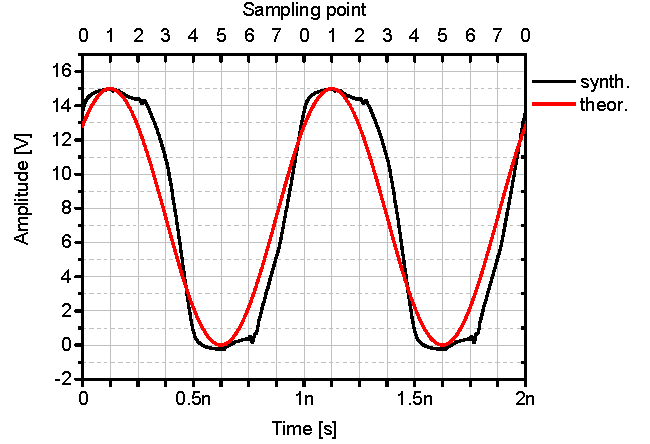
\includegraphics[width=0.75\textwidth]{Vout_SynthVsTheo.pdf}
   \caption{Synthesized sine wave with the theoretical sine wave}
   \label{fig:SineWaveSynthVsTheoretical}
\end{figure}
% 03:12 Uhr 29.04.2016
Although the synthesized signal is clipped and the mentioned distortion came into play, the shape looked like a sine wave.
The \gls{ab:snr} of the synthesized signal was calculated with MatLab and was $SNR = 15$\si{\decibel}.
For a first evaluation of the signal quality after digital-to-analog conversion, the spectra were compared.
The spectrum of a time signal demonstrates the frequency portions which are present in the signal.
As the spectrum of a clear sine wave only consist of a \gls{ab:dc} component and its first harmonic, it was easy to obtain a comparable quantity compared to the synthesized signal.
Figure \ref{fig:SineCompare} highlights the difference between the synthesized and the theoretical sine wave form in more detail.

\begin{figure}[htb!]
	\centering
  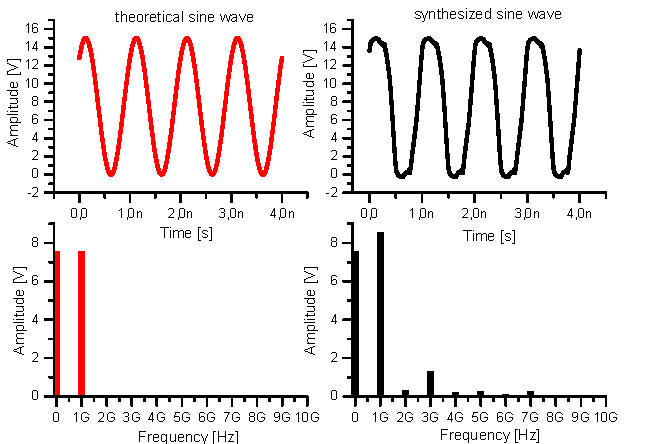
\includegraphics[width=1\textwidth]{SineCompare3.pdf}
	\caption{Comparison between a theoretical and a synthesized sine wave with their spectrum}
	\label{fig:SineCompare}
\end{figure}

On the top left side the theoretical sine wave is plotted in time domain. 
Underneath of it the spectrum presented a frequency portion for the direct component at \SI{0} {\Hz} and a fundamental frequency portion at \SI{1}{\GHz}. 
The spectrum of the synthesized sine wave on the top right side demonstrates a few distortions at higher frequencies.
Beside the direct and fundamental frequency component there were some additional unwanted frequency portions which distorted the signal.
The comparison of the spectra was a good indicator for a first error estimation.
This optical measure made it easy to evaluate the signal quality since the unwanted distortions were clear visible.
At the third harmonic the signal deviates by 14\% from the clear sine, as for the 2nd to 10th harmonic the deviation is up to 7\%.
As already mentioned the calculated \gls{ab:snr} was \SI{15.2}{\decibel} of a theoretical achievable \SI{27}{\decibel}, since this signal was scaled for the full scale.
Compared to a full scale sine wave, a \gls{ab:snr} of \SI{22}{\decibel} could be achieved for a frequency of \SI{1.5}{\giga \hertz} with the presented Riemann Code in equation \ref{eq:RiemannCodeSineWave}.
Figure \ref{fig:SNRSine1.5GHz} demonstrates this synthesized signal with its \gls{ab:snr}.

\begin{figure}[htb]
	\centering
  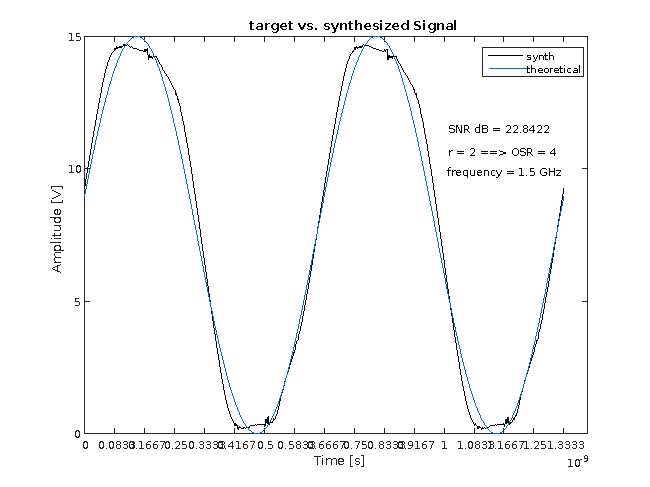
\includegraphics[width=0.9\textwidth]{FullSine15GHz.pdf}
	\caption{calculated SNR for frequency of 1.5 GHz}
	\label{fig:SNRSine1.5GHz}
\end{figure}

Further details on the \gls{ab:snr} calculation for various signals, can be found in appendix \ref{app:snr}.
In addition to tune the amplitude via the absolute sampling intervals, it was also possible to adapt the input control sequence, hence the sequence of chosen slopes to shape the output signal.
The three bit resolution restricted the quantity of different slope combinations to six for synthesizing a sine wave.
Considering only two sampling intervals to construct the rising edge of the positive half sine, the six combinations were: 75, 73, 71, 53, 51 ,31 with respect to the $i_0$ values.
As these relative slopes were used for the rising edge, the counterparts (negative values) represent the falling edge.
The first digit indicated the slope of the first sampling interval and the second digit of the second, respectively. 
These six combinations were plotted in Figure \ref{fig:SameSigBWDifSlope} over two periods for the signal frequency of \SI{3}{\GHz}. 

\begin{figure}[htb!]
	\centering
  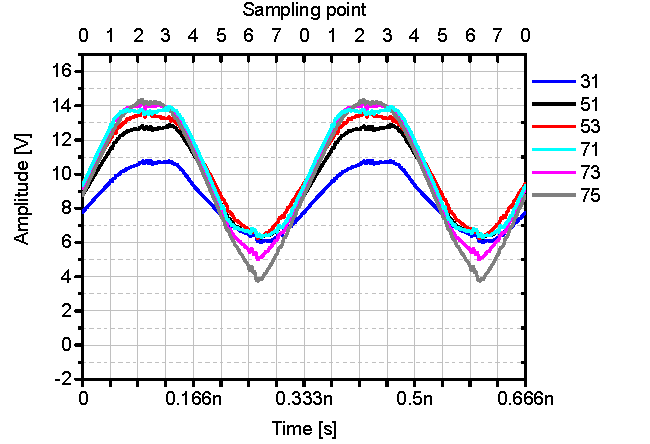
\includegraphics[width=.75\textwidth]{Vout_7sine_SameSigBWdifferent_DifferentSlope.pdf}
	\caption{Signals with the same signal bandwidth \SI{3}{\giga \hertz} but different input control}
	\label{fig:SameSigBWDifSlope}
\end{figure}

Here the effect of the Riemann Code became clear, since the change of the input control will also change the shape of the output signal.
This was utilized to calculate the Riemann Code with an algorithm to fit the output to the desired signal.
The algorithm had to be processed within the settling time of the \gls{ab:dac} to ensure real time conversion.

\subsection{Full wave rectified sine wave generation in the time domain}
In addition to the sine wave, here a full wave rectified sine wave was simulated.
Based on the same approximation principle as demonstrated in figure \ref{fig:RiemannCodeGenerationSineWave}, the corresponding Riemann Code for the rectified sine was generated and is stated in equation \ref{eq:RiemannCodeRectSine}.

%% THIS CORRESPONDS TO 7 5 3 1 -1 -3 -5 -7 
%% SINCE THIS IS ENOUGH TO SYNTHESIZE A PERIOD
\begin{equation}
 000\hspace{.3cm} 001\hspace{.3cm} 010\hspace{.3cm} 011\hspace{.3cm} 100\hspace{.3cm} 101\hspace{.3cm} 110\hspace{.3cm} 111.
\label{eq:RiemannCodeRectSine}
\end{equation}

As the rectified sine wave consisted only of the positive wave for a full period, the oversampling ratio is performed on half of a sine wave.
This resulted in a more precise wave form which resulted in an \gls{ab:osr} of eight (r=3) compared to the full sine wave.
Here the number of slopes used for synthesizing the rising edge was doubled and hence four different slopes could be used.
Therefore the rectified sine wave consisted of eight sampling points, while the corresponding positive half of a sine wave only consisted of four sampling points.
The rectified sine wave exhibited the sequence of all eight different slopes, from the biggest positive to the biggest negative slope.\\
Signals in the frequency range of \SI{500}{\mega \hertz} to \SI{6}{\giga \hertz} were generated and  are demonstrated in Figure \ref{fig:DiffSigBWSameSlope}.

\begin{figure}[htb!]
	\centering
  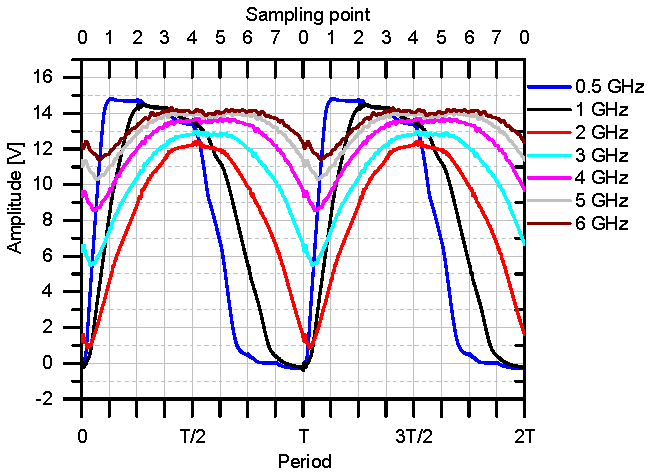
\includegraphics{Vout_halfsine_7531_diff_freq.pdf}
	\caption{Signals with same slope but different signal bandwidth}
	\label{fig:DiffSigBWSameSlope}
\end{figure}

The shapes of the signals with fundamental frequencies \SI{2}{\giga \hertz} to \SI{6}{\giga \hertz} fit very good to a rectified sine..
The issue of signal clipping was the same as mentioned earlier.
This effect was seen in Figure \ref{fig:DiffSigBWSameSlope} for the blue curve which had a fundamental frequency of \SI{500}{\mega \hertz}.
Further investigations on the \gls{ab:snr} were omitted due to the limited scope of this thesis.

\subsection{Triangular wave generation in the time domain}
As the designed circuit should act as a signal generator another signal was synthesized.
A triangular signal was chosen to validate the feasibility of generating arbitrary waveforms.
The wave form of a triangular signal is generated by charging and discharging a capacitor for the same period of time.
All simulations so far, were run with a three bit resolution of the realised circuit.
This three bit resolution represented eight different slopes and therefore for a equally charge and discharge process four different slopes could be used.
These four slopes were +7, +5, +3, +1 for the charging process and their counterparts -7, -5, -3, -1 for discharging.
Hence the sequences of slopes were: 77,55,33 and 11 with respect to $i_0$ values.
Figure \ref{fig:DiffSlopeSameBWTriangular} demonstrates the four different combinations for synthesizing a triangular wave form for \gls{sy:fsignal} = \SI{2}{\giga \hertz}.

\begin{figure}[htb!]
	\centering
  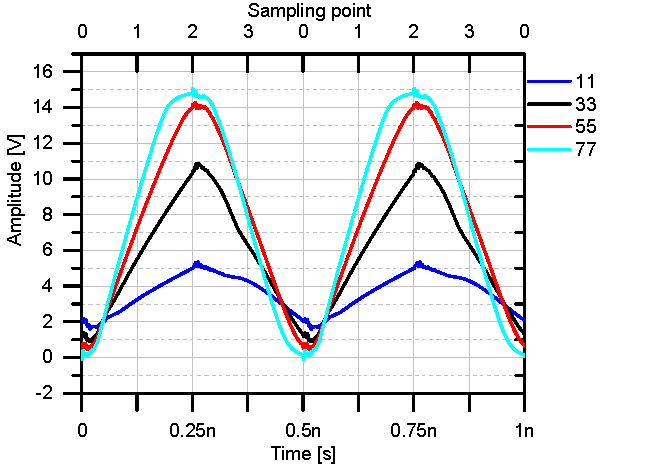
\includegraphics{Vout_triangular_2GHz_diffSlopes.pdf}
	\caption{Triangular signal with same signal bandwidth but different slopes}
	\label{fig:DiffSlopeSameBWTriangular}
\end{figure}

The fundamental frequency was set to \SI{2}{\giga \hertz} representative for the signals with \gls{sy:fsignal} in the frequency range of \SI{500}{\mega \hertz} to \SI{6}{\giga \hertz}.
In this configuration only the wave form for the biggest slope (77; cyan) deviates from the desired signal.
At the sampling point 2 the output capacitance is fully charged which led to an undesirable signal form.
In fact of the high current and long sampling interval, the output capacitor is fully charged.
The problem of not defined reference currents can be observed in the following calculation.
For a reference current $i_0$ of approximately \SI{160}{\milli \ampere}, a capacitance $C$ of \SI{20}{\pico \farad} and a sampling interval $dt$ of \SI{125}{\pico \second} the voltage swing can be calculated as:
\begin{equation}
	dU = \frac{7 i_0*2 dt }{C} = 14 V,
\end{equation}

which fit pretty good to the cyan signal in Figure \ref{fig:DiffSlopeSameBWTriangular}.
Taken the same parameters for the slopes of $5 i_0$, $3 i_0$ and $1 i_0$ it follows a voltage swing of $dU = 10 V$, $dU = 6 V$ and $dU = 2 V$ respectively.
The reason this voltage swings could not be observed in Figure \ref{fig:DiffSlopeSameBWTriangular} is due to the problem of not perfectly defined current sources. 
Representative for the four combinations to synthesize this triangular signal wave form, 
Figure \ref{fig:DiffSigBWSameSlopeTriangular} demonstrates the frequency varying signals from \SI{500}{\mega \hertz} to \SI{6}{\giga \hertz} for a slope of 33.


\begin{figure}[htb!]
	\centering
  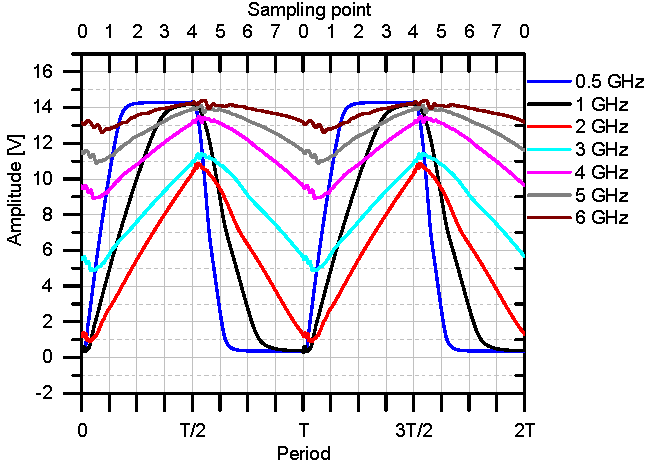
\includegraphics{Vout_triangular_Slope33_diffFreq.pdf}
	\caption{Triangular signal with same slope but different signal bandwidth 3GHz}
	\label{fig:DiffSigBWSameSlopeTriangular}
\end{figure}

%The Code for the generation of the triangular signal at the output is:
%\textbf{this is not the correct code!!}
%\begin{equation}
% 000\hspace{.3cm} 010\hspace{.3cm} 101\hspace{.3cm} 111\hspace{.3cm} 000\hspace{.3cm} 010\hspace{.3cm} 101\hspace{.3cm} 111.
%\end{equation}
%\label{eq:RiemannCodeRectSine}

% short definition of stability, what cause oscillation, how to measure stability -> plot stability circles for the schematic%
\section{Stability analysis of the realised circuit}
To guarantee a proper function of the circuit a short stability analysis was performed.
This analysis was necessary to check if the circuit oscillates.
To prevent the circuit to take damage this oscillation had to be avoided.
It was checked if the \gls{ab:dut} was stable for the whole frequency range used.
Using a S-parameter simulation the complex impedance at various critical points was calculated.
One condition to start an oscillation is a feedback path which existed for the designed circuit.
The driver circuit for the high side switch is connected to the output and hence the feedback is established.
To avoid unwanted oscillation the real part of the complex impedance had to be positive for the whole frequency range.
A basic definition of passive elements were that they have a reflection coefficient magnitude less than unity.
Checking the input reflection coefficient, the values had to be inside the unity circle.
Therefore no negative resistance would be allowed to occur since that can lead to unwanted amplification and oscillation which can damage the circuit \cite{GilmoreR.2003}.
Because the real part of the impedance at all measurement points were positive for the whole frequency range, the circuit seemed to be stable.
The stability check was performed within the \gls{ab:ads} tool. 

\section{Power consumption analysis of the realised circuit}
As the concept is designed for the purpose to implement in mobile communication systems the power consumption is crucial.
Since the energy storage of mobile devices is limited, it is important to get a decent power dissipation for the test circuit.
A short analysis should give an insight to the expected power consumption of the designed test circuit.
Due to the expected switching losses \cite{Quay2014}:
%$ P_{cond} = R_{DS,on}dI_0^2 \propto R_{DS,on} $ \\
\begin{equation}
 P_{sw} = \frac{1}{2} V_{in}I_0(t_{on}+t_{off})f_{sw} \propto f_{sw}
 \label{eq:swtichloss}
\end{equation}

the power consumption scales linear with the switching frequency, here \gls{sy:fsampling}.
Simulations confirmed this assumption for switching the smallest bit of the Riemann Pump.
The used input code was a sequence of alternating bits, since its a different power consumption for switching $+1 i_0$ than for $-1 i_0$.
Switching the high side transistor to the off state results in a leakage current over the high sides driver circuit.
A trade off between switching speed and power consumption resulted.
For an increase in the switching speed, hence an increase of the signal bandwidth, the power consumption also linearly increase.
In addition to this, the power consumption of the driver circuit also increases with the switching speed, as the dimensions of the used components have to be adapted.
The used driver circuit was optimized to reduce the power consumption for a maximum frequency of \SI{100}{\mega \hertz}, as it was implemented in a power application system \cite{MaksimovicPaper}.
The estimated losses are illustrated in Table \ref{tab:switchloss} with the corresponding sampling (switching) frequency of the used configuration.

\begin{table}[ht]
\centering
\begin{tabular}{|l|l|}
\hline
$f_{sampling}$ {[}GHz{]} & $P_{diss}$ {[}W{]} \\ \hline
4                    & 3.982              \\ \hline
8                    & 4.259              \\ \hline
16                   & 4.778              \\ \hline
24                   & 5.011              \\ \hline
32                   & 5.144              \\ \hline
40                   & 5.264              \\ \hline
48                   & 5.354              \\ \hline
\end{tabular}
\caption{Overall power losses for sampling rate}
\label{tab:switchloss}
\end{table}

The used configuration referred to the one bit Riemann Pump consisted of two power transistors, for the high and low side switch, with a gate periphery of \SI{800}{\micro \meter}, four driver transistors each with \SI{200}{\micro \meter} gate periphery and the bias voltages of \gls{sy:vdn} = \SI{-5}{\volt}, \gls{sy:vdp} = \SI{0}{\volt} and \gls{sy:Vdd} = \SI{15}{\volt}.
This configuration can be seen in appendix \ref{app:schematic} on the right hand side.
%As stated in the fundamentals the energy consumption for a dac with 17 ENOB and a sampling rate of 10G will result in several kilo watts, this dac also consumed so much. As the following bits, here power transistors scale with a factor of two it yielded a consumption for 17 bit at 10 G of: sum(2^i), i =0:16 = 131071 i0 = 131071*4W = 400kW --> reference to DAC used in the paper for fig 2.2

\newpage
\section{Proof of concept simulation with existing components}
\label{ch:ProofOfConceptWithExistingComponents}
In the last step a simulation was run which made the concept comparable to the realized circuit. 
The realized circuit was designed with the help of former designed chips.
In this simulation the transistor dimensions were adapted to the dimension of the built demonstrator. 
This should give an insight to the behaviour of the constructed demonstrator.
The detailed modelling and simulation of the designed circuit under real conditions, considering all loss effects would go beyond the scope of this thesis, since no models for the used chips were available.
As the realized demonstrator differs slightly from the presented concept, Figure \ref{fig:democircuit} demonstrates the circuit schematic for one bit.
\begin{figure}[htb!]
	\centering
  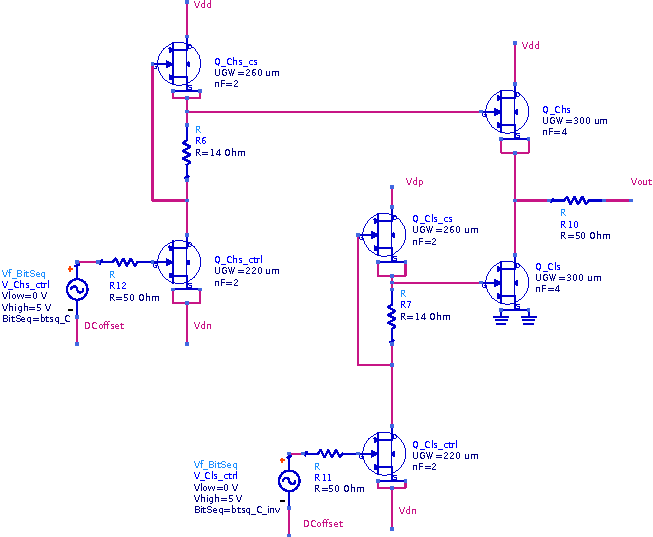
\includegraphics[width=\textwidth]{realizedCircuit_oneBit_DDRi_XY6.pdf}
	\caption{demo circuit}
	\label{fig:democircuit}
\end{figure}

The difference to the presented concept was that no feedback path from the output to the drain of the high side driver circuit existed.
The result of this was that the efficiency was not as good as for the presented concept in chapter \ref{ch:design}.
It is to mention that the transistors for the other bit scales with the factor 2.
The full schematic of the built demonstrator circuit can be seen in Appendix \ref{app:schematicRealizedPump}.
Although the used chips for the demonstrator were designed in a former work, no simulation files were available which made a detailed simulation difficult.
Nevertheless this built circuit acted as expected and a signal could be synthesized, as seen in Figure \ref{fig:sim}.

\begin{figure}[htb!]
	\centering
  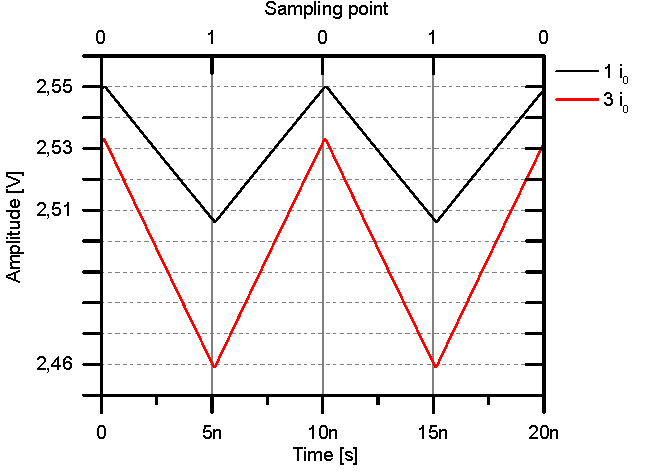
\includegraphics{SimulationForMeasData.pdf}
	\caption{Simulation result for the output voltage using the realized components}
	\label{fig:sim}
\end{figure}

As the measurement of the time signal was performed with an oscilloscope and a probe, the load impedance differs from the concept.
Figure \ref{fig:equivalentprobecircuit} in Chapter \ref{ch:timedomainmeas} presents the equivalent circuit for the measurement.
Considering this, gave the simulation results presented in Figure \ref{fig:sim} which demonstrates the signal generation.
The black signal represents a triangular waveform with a relative slope of $1 i_0$ and the red of $3 i_0$, respectively.
The voltage swing is $0.04 V$ and $0.07 V$ since the probe divides the real voltage with a ratio of 10:1 to avoid any damage of the oscilloscope.
Therefore the real voltage swing is $0.4 V$ and $0.7V$ which fit pretty good to the measured data in chapter \ref{ch:timedomainmeas}.
The simulation is run with the circuit in Figure \ref{fig:democircuit}, a load impedance corresponding to the measurement in Figure \ref{fig:equivalentprobecircuit} in Chapter \ref{ch:timedomainmeas}, \gls{sy:fsampling} of \SI{200}{\mega \hertz} and $V_{dn} = -5V, V_{dp} = 0V, V_{dd} = 5V$.



% As DDRi2C is used, bottom vdp(in na; lowside) = vdd. 
\newpage
\section{Evaluation of the simulation results for the Riemann Pump}
Different wave forms could be synthesized (sine wave, rectified sine, triangular).
The dimension of the used components already limits the bandwidth.
To shift the bandwidth to higher values the transistor dimension have to be bigger and smaller to shift to lower values, respectively.
The signal frequency of \SI{1}{\giga \hertz} represented a lower bound on the frequency range in the used configuration.
With an \gls{ab:osr} of four \gls{sy:fsampling} is eight times \gls{sy:fsignal}.
The smallest achievable current times the smallest sampling time (highest sampling frequency) determine the smallest voltage step achievable.
If the \gls{ab:osr} is increased, the sampling time is decreased and therefore the signal quality is better because we have a more accurate synthesized signal. 
The upper bound of the frequency range is limited to the detectable voltage swing of the amplitude.
In addition to this the components have a unity current gain frequency limit.
Higher frequency means much lower sampling time which can lead to non detectable voltage steps (slopes are not detectable).
Parasitic and loss effects distorted the waveforms.
Since the digital to analog conversion always introduces noise to the signal the fit was not perfect.
The highest \gls{ab:snr} (\SI{32.5}{\decibel}) found was for a sine wave at \SI{6}{\giga \hertz} with an amplitude of $\hat{v} = 1.75 V$, an DC-offset of $V_{DC} = 13 V$ and a phase shift of $\phi = -\pi/8$, see appendix \ref{app:snr}.
There are the \gls{ab:snr} values presented for the seven different signals of Figure \ref{fig:7SignalsSameSlopeInOnePlot} with their corresponding theoretical wave form parameters.
The system is stable.
The stability check was needed to validate that the circuit did not oscillate.
The energy consumption is in the range for base stations and have not reached it yet for mobile devices.
Since the resolution should be in the range of 17 bits.
If the resolution is increased to get a better accuracy, the whole circuit would become more complex and the energy consumption would increase.
If the \gls{ab:osr} is increased to get a better accuracy, the switching frequency is also increased and therefore the energy consumption.
For high switching frequencies the switches have to switch within a few \si{\nano \second} which increase the gate drive current which increase the power loss.
This is the trade off between the shift of the bandwidth (shifting to even higher frequencies is possible but the bandwidth is nearly constant) and power consumption.
The designed test circuit is not optimal with respect to efficiency.
The implemented driver circuit absorbed unexpected leakage currents.\\
Nevertheless the simulation results confirmed the feasibility of the chosen approach.
Some trade-offs in mind and the ability to change some system parameter made it possible to generate some good fitted signal waveforms.
\chapter{Realisation of a Riemann Pump circuit}
\textit{Outline of the technologies used to fabricate and assemble your structures, if applicable. Detailed processes belong in the appendix. If numerous types of structures were fabricated, or assembly technology is extensive, there may be more than one of these chapters. \textbf{Characterization} Description of the means developed and employed to characterize the devices or systems that have been fabricated.}
Design of the rogers 4003P substrate. Filter network, chip placement, bond, input output connectors everything. Difficult to layout the PCB, because no special frequency is desired. It is a whole bandwidth and thus it makes it difficult to tune the board. So many factors come into account. Bypass, decoupling capacitors for a great bandwidth instead of a special frequency. 
\begin{itemize}
	\item bypass cap dimension
	\begin{itemize}
		\item large package - more inductance - lower freq
		\item higher ESR - bad quality factor - flatten mag of imp vs. freq - broadband good
		\item temp range, voltage range, tolerance, 
		\item dimension: cargo cult principle - rule of thumbs
	\end{itemize}
	\item DC blocking, filter caps (not used) 
	\item bias tees to add bias 
	\item no dc input line because of the bias tee
	\item metal pad size of chip
	\item thermal conduction, dissipate the heat
	\item line distance
	\item line width, copper height, substrate height, determine the impedance of the msl
	\item no qfn package because the heat would not be dissipated
	\item input line - 50 ohm lines
	\item mmic caps near to the supply pin
	\item equal distance of bonds
	\item bond diameter?
	\item via holes for thermal conduction
	\item backside of chips are metallized
	\item equal length of input lines
	\item 50 ohm output line
	\item metal pad size of chip vs. distance to another pad with vias
	\item coupling could be a problem
	\item sma connector to attach measurement devices
	\item DC power supply with -5V means that ground is 5V
	\item two different layouts
	\begin{itemize}
		\item chip with gnd vias on island and nearby copper plate with thermal vias to cool down the ambient temp of the MMIC
		\item chip without gnd via, direct soldered on the copper with thermal vias
	\end{itemize}
\end{itemize}

Design is ordered 22nd of Feb at contag.de in Berlin.
Also Digikey parts were ordered the week before, 15-19.02 in the Netherlands. A Saegeauftrag were ordered at Axel Tessmann and M. Zink, Riessle. 
\chapter{Measurement results}
\textit{The heart of the thesis, comprising a presentation of the functioning system and thus the culmination of the work. Important is an analysis of the results as well as a comparison with the state of the art. The reader should understand in this section why you should be awarded a MSc degree.}
\section{Measurement setup}
This section will describe the measurements. First of all an overview of the setup is given. Then the calibration and measurement is described and last but not least the results are discussed. The test setup is resort by an former work.
Input control and output measurement are key factors. The input is controlled by an AWG from Keysight, programmed with a determined data set of bits. Based on the work of Stephan Maroldt, some MMICs were taken to to realise the desired schematic. 
\begin{itemize}
	\item Keysight AWG - (1V := 0dB; 0.7V := -3dB)
	\item Broadband (35kHz-40GHz) amplifier (17dB gain) (digital signal with clk 1GHz, 10 harmonics -> 10GHz)
	\item Bias Tees (DC bias)
	\item DC supply (driver network, power transistor)
	\item DUT
	\item LOAD - OUTPUT ???
\end{itemize}
Output measurement maybe with anteverta active load pull system. Another option would be to scope a real time output on-wafer with an oscilloscope.
\section{Measurement results}
\subsection{comparison of simulation versus measurement}
how to measure at the output of the schematic? is the measurement result as expected from the simulation?
\subsection{limitations and prolems with measurement}
\chapter{Conclusions and outlook}
\textit{A summary of the most important results, whereby a repeated emphasis of their relevance, importance and novelty cannot hurt. A brief precis of the envisaged future potential of the work is suitable here, but avoid addressing the Nobel Committee directly.}
The calculation of the Riemann Code have to be done with an external signal processor, which has to compute this code in real time. 
This could be a problem, since the energy consumption could increase and the real time calculation.
%Nonetheless the number of signals which can be synthesized with this particular concept is increased with the possibility to change to another combination of slopes to approximate the signal.
%All this calculation should be done with a signal processor and an algorithm.
%With the variation of the slopes and the variation of the sampling time in theory it is possible to create every single signal with more or less good \gls{ab:sqnr}.
 In a more enhanced project a MATLAB algorithm would compute this code by minimizing the deviation between a theoretical signal and the synthesized signal.

\nocite{Devrac2014}
\nocite{Devrac2015}


\cleardoublepage
\clearpage
\phantomsection

%\addcontentsline{toc}{chapter}{\bibname}
\bibliographystyle{IEEEtran}
%\clearscrheadings
%\manualmark
%\markboth{Literature}{Literature}
\bibliography{literature}

%\printglossary[title=List of Symbols, style=long]
%
%\printglossary[type=\acronymtype, title=List of Abbrevations, style=long]
\renewcommand*\thechapter{}
\renewcommand*\thesection{\Alph{section}}
\chapter*{Appendix}
\chaptermark{Appendix}
\stepcounter{chapter}
\ifoot{Appendix}
\addcontentsline{toc}{chapter}{Appendix}

\section{Schematic of the Riemann Pump circuit}
bla bla bla bal bla lbal blalsl

\newpage
\section{Layout of the whole Riemann Pump circuit}

bla bla bla bal bla lbal blalsl

bla bla bla bal bla lbal blalsl

\newpage
\section{Photography of the realized Demonstrator version 1}

bla bla bla bal bla lbal blalsl
\section{Photography of the realized Demonstrator version 2}

bla bla bla bal bla lbal blalsl
%\cleardoublepage
%$\markboth{\nomname}{\nomname}
\cleardoublepage
%\Declaration

%\makeiheabstract

% Anhang/Appendix
%\begin{appendices}
%\renewcommand{\appendixtocname}{Anhang}
%\renewcommand{\appendixname}{Anhang}
%\addappheadtotoc
%\appendixpage
%\end{appendices}

\end{document}



	%\begin{tabular}{ll@{\hspace{1cm}}ll@{\hspace{1cm}}l}
